\documentclass[journal]{IEEEtran}

\usepackage[T1]{fontenc}
\usepackage{newtxtext,newtxmath}
\usepackage{cite}
\usepackage{array}
\usepackage{booktabs}
\usepackage{tabularx}
\usepackage{multirow}
\usepackage{graphicx}
\usepackage{xcolor}
\usepackage{tikz}
\usetikzlibrary{positioning,arrows.meta,fit,calc,backgrounds,patterns}
\usepackage{pgfplots}
\pgfplotsset{compat=1.18}

\newcolumntype{L}[1]{>{\raggedright\arraybackslash}p{#1}}
\newcolumntype{Y}{>{\raggedright\arraybackslash}X}

\begin{document}

\title{Toward Privacy-Preserving Detection of Trade-Based Money Laundering: A Systematic Review of Graph Learning, Federated Learning, and Blockchain Auditing}

\author{Anuj Nanhe, Aniket Shelke, Laiba Shaikh, and S. R. Khonde}

\markboth{SYSTEMATIC REVIEW}{SYSTEMATIC REVIEW}

\maketitle

\begin{abstract}
Money laundering through bank transfers and through international trade is hard to detect because the evidence is split across institutions that cannot share raw customer data. Graph learning, federated learning, and blockchain are each proposed as part of the answer, but they are studied by separate communities. This paper presents a systematic review of how these techniques are used to detect laundering and financial fraud, how they protect the data of the participating institutions, and how they make detection auditable. Following PRISMA 2020, 34 full-text files collected from IEEE Xplore and Emerald Insight in four thematic clusters were screened. After duplicates were removed and one unretrievable report was set aside, 27 studies were assessed in full text, and all were retained and classified against a taxonomy of seven categories. Graph models report strong results on the Elliptic Bitcoin data and on the synthetic IBM transactions, but datasets, splits, and metrics differ so much that the numbers cannot be ranked. Only three studies train fraud detectors across institutions with federated learning. None of them uses laundering data, and the only one that lets institutions keep different columns without matching customers has two clients. Secure aggregation hides individual updates, yet one study shows that it still reveals which classes a participant holds. In a federation of banks this could expose the banks that hold confirmed laundering cases. Blockchain is used for incentives, accountability, policies, and documents, but no study records the updates and alerts of a detection model on a ledger. The literature on trade-based laundering offers price statistics, mirror analysis, and a single classification study. We synthesize these findings into a taxonomy, ten research gaps, and a reference architecture for privacy-preserving and auditable detection across banks, with trade data as the next step.
\end{abstract}

\begin{IEEEkeywords}
Anti-money laundering, trade-based money laundering, federated learning, secure aggregation, graph neural networks, blockchain, explainable AI, financial fraud detection, systematic review.
\end{IEEEkeywords}

\section{Introduction}

\IEEEPARstart{M}{oney} laundering moves the proceeds of crime into the legitimate economy. Estimates attributed to the United Nations Office on Drugs and Crime put the amount laundered each year at 2\% to 5\% of world GDP, or about USD 800 billion to 2 trillion \cite{raj2024ai}, and a review focused on banks quotes 2.1\% to 4\% of the world economy \cite{jensen2023fighting}. Banks are required to know their clients and to monitor and report suspicious behavior. Most monitoring still runs on rules written by experts. The rules are easy to read but inefficient, and over 98\% of AML alarms can be false positives \cite{jensen2023fighting}. Banks receive little feedback on the reports they file, and launderers change their behavior once they learn how they are being watched \cite{jensen2023fighting}.

Laundering is not limited to bank transfers. In trade-based money laundering (TBML), value is moved by misrepresenting the price, quantity, or quality of imports and exports \cite{fatf2006tbml,tiwari2025tbml}. Goods can be invoiced above or below their fair price, more or less can be shipped than is declared, and the quality of goods can be misstated. Services are harder to price, so the same service can be invoiced several times \cite{tiwari2025tbml}. Detecting such schemes requires matching invoices, shipping records, customs declarations, and payments that are kept by different organizations.

In both cases the evidence is split. A launderer spreads transfers over several banks, and each bank sees only its own part of a payment chain. Each bank also stores different information about its customers. Data protection law prevents institutions from pooling customer data in one place \cite{awosika2024xai}. The detection studies in this review therefore train on the data of a single institution or case \cite{irshad2024gcfmld,luo2024mlad}, on public data whose features are anonymized and poorly documented \cite{ferretti2025gnn}, or on synthetic data \cite{mao2026pmegnn,amber2026cbdc}.

Three families of techniques address parts of this problem. Graph learning uses the structure of payment networks, which carries information that a single transaction lacks \cite{ferretti2025gnn,mao2026pmegnn,yu2023aetransgat}. Federated learning (FL) lets institutions train one model while each keeps its data \cite{mcmahan2017fedavg}, and secure aggregation hides the update of each participant from the server \cite{bonawitz2017secagg}. Blockchain keeps a shared record that cannot be changed once written and that several parties can check, which suits audit trails for regulators \cite{chen2024finance} and accountability among FL participants \cite{yang2022accountable}. These families are studied by different communities. The graph studies in this review train on data held in one place, the FL studies use card and account fraud data rather than laundering data, and the blockchain studies rarely evaluate a detector.

Existing reviews cover parts of the problem. Jensen and Iosifidis review statistical and machine learning methods for AML in banks and call for public data, semi-supervised learning, and interpretable models, but they do not discuss collaboration between banks \cite{jensen2023fighting}. Tiwari et al. give the first systematic review of TBML and find that the detection literature is too small to say which methods work \cite{tiwari2025tbml}. Ahmed and Alabi review FL built on blockchain for detecting cryptocurrency fraud \cite{ahmed2024bcfl}. Other surveys cover FL on a blockchain in general \cite{li2021befl}, blockchain as a platform for machine learning \cite{ural2023bcml}, and blockchain in finance \cite{chen2024finance}. None of them asks how the three families fit together for detection across institutions, or what is missing before they can be applied to trade.

This review addresses that gap through a systematic analysis of 27 studies on laundering and fraud detection, FL and its protections, and blockchain support for learning and financial records. Its contributions are as follows:
\begin{enumerate}
\item A systematic review of 27 studies from IEEE Xplore and Emerald Insight that follows PRISMA 2020 \cite{page2021prisma}. Each study is classified by primary category and relevance, and the complete classification is given in the Appendix.
\item A taxonomy that places data sources, graph representations, detection models, collaboration schemes, protection mechanisms, and audit layers in one pipeline (Fig.~\ref{fig:taxonomy}).
\item A comparison of the reported detection results that shows where the numbers can and cannot be compared (Section~\ref{sec:rq1}).
\item An analysis of FL for financial fraud and of secure aggregation, including the attacks that remain open (Sections~\ref{sec:rq2} and \ref{sec:rq3}).
\item An account of how blockchain and explanation methods support auditing (Sections~\ref{sec:rq4} and \ref{sec:rq5}) and of what the TBML literature offers (Section~\ref{sec:rq6}).
\item Ten research gaps and a reference architecture for privacy-preserving and auditable detection across banks, with an extension to trade data (Sections~\ref{sec:gaps} and \ref{sec:arch}).
\end{enumerate}

The rest of the paper is organized as follows. Section~\ref{sec:background} gives background and compares related reviews. Section~\ref{sec:method} describes the review protocol and Section~\ref{sec:corpus} characterizes the corpus. Sections~\ref{sec:rq1} to \ref{sec:rq6} answer the six research questions. Section~\ref{sec:gaps} sets out open research gaps and Section~\ref{sec:arch} proposes a reference architecture and research agenda. Section~\ref{sec:validity} discusses threats to validity and Section~\ref{sec:conclusion} concludes.

\section{Background and Related Reviews}
\label{sec:background}

\subsection{Money Laundering and Its Detection}

Laundering is usually described in three stages \cite{raj2024ai,irshad2024gcfmld}. In placement, illicit funds enter the financial system, often split into many small deposits. In layering, they are moved through a series of transactions and accounts to hide their origin. In integration, they return to the economy as apparently legitimate wealth. Jensen and Iosifidis divide AML work in banks into two tasks \cite{jensen2023fighting}. Client risk profiling assigns each client a general risk score, for example during know your customer (KYC) checks. Suspicious behavior flagging raises alarms on clients, accounts, or transactions during monitoring. Analysts review the alarms, and the cases they confirm are reported to the authorities as suspicious activity reports (SARs) \cite{irshad2024gcfmld}.

The labels that detection models learn from come out of this process. A case counts as laundering when an analyst escalates it, so labels are scarce, arrive late, and depend partly on judgment \cite{jensen2023fighting,irshad2024gcfmld}. Public data are scarce for the same reason. Three public datasets recur in the corpus. The Elliptic dataset is a graph of 203{,}769 Bitcoin transactions and 234{,}355 flows between them, with 166 features per transaction. Only 4{,}545 transactions are labeled illicit and 157{,}205 are unlabeled \cite{weber2019elliptic,yu2023aetransgat}, and the meaning of most features is not documented \cite{ferretti2025gnn}. The IBM AML datasets are produced by a simulation of interacting agents that injects known laundering patterns into ordinary activity \cite{altman2023ibmaml}. Their HI-Small subset holds about 5 million transfers between 515{,}000 accounts over ten days, and one transfer in 981 is laundering \cite{mao2026pmegnn}. EthereumHeist traces more than 160{,}000 addresses downstream of 73 security incidents on Ethereum \cite{wu2024heists}. Other studies use the private data of a bank \cite{irshad2024gcfmld}, data from a law enforcement case \cite{luo2024mlad}, or synthetic data generated for the study \cite{amber2026cbdc}.

TBML moves value through trade rather than through transfers alone. The Financial Action Task Force (FATF) defines it as disguising the proceeds of crime by moving value through trade transactions and misrepresenting the price, quantity, or quality of imports or exports \cite{fatf2006tbml}. Zdanowicz studied abnormal prices in trade statistics as a sign of illicit transfers between countries \cite{zdanowicz2009}. The records needed to detect TBML are held by banks, traders, shipping companies, and customs authorities, and these records are rarely joined \cite{tiwari2025tbml,dudczyk2024supply}.

\subsection{Federated Learning and Its Protections}

In FL a server sends a global model to the participants, each participant trains it on its own data, and the server averages the returned parameters, weighting each participant by its number of samples \cite{mcmahan2017fedavg}. This algorithm is called FedAvg. Two settings matter for financial crime \cite{li2026plc}. In horizontal FL the participants hold the same features for different customers, as banks of the same kind do. In vertical FL they hold different features for the same customers, for example a bank and an online shop, and they must first match their customer identifiers through private set intersection. Records that do not match are then discarded \cite{li2026plc}.

Sharing parameters instead of data does not make FL private by itself. Gradients can be inverted to reconstruct inputs, and model updates support membership inference and model inversion attacks \cite{li2026plc,sami2024tinysecagg}. Three kinds of protection appear in the corpus. Differential privacy adds noise to the updates and costs accuracy \cite{li2026plc}. Homomorphic encryption lets the server aggregate encrypted models, but it is computationally heavy \cite{xiong2025hppbefl}. Secure aggregation masks each update with random values that cancel in the sum, so the server learns only the aggregate \cite{bonawitz2017secagg,sami2024tinysecagg}.

\subsection{Related Reviews}

\begin{table*}[!t]
\centering
\caption{Reviews and Surveys Within the Corpus Compared With This Review}
\label{tab:reviews}
\footnotesize
\begin{tabularx}{\textwidth}{@{}L{1.05cm}YL{2.6cm}L{2.05cm}L{1.9cm}L{1.55cm}L{1.55cm}@{}}
\toprule
\textbf{Review} & \textbf{Focus} & \textbf{Corpus} & \textbf{Detection models} & \textbf{Learning across institutions} & \textbf{Blockchain} & \textbf{TBML}\\
\midrule
\cite{jensen2023fighting} & Statistical and machine learning methods for AML in banks & Narrative & Yes & No & No & No\\
\cite{raj2024ai} & AI across KYC, due diligence, and monitoring & Narrative & Conceptual & No & No & No\\
\cite{tiwari2025tbml} & TBML literature & 33 records and 214 found by citation mapping & Price and mirror statistics & No & No & Yes\\
\cite{ahmed2024bcfl} & FL built on blockchain for cryptocurrency fraud & Not stated & Partial & Yes & Yes & No\\
\cite{li2021befl} & FL on a blockchain & Narrative & No & Yes & Yes & No\\
\cite{ural2023bcml} & Blockchain as a platform for machine learning & Narrative & No & Partial & Yes & No\\
\cite{chen2024finance} & Blockchain in finance beyond cryptocurrency & Narrative & No & No & Yes & Partial\\
\cite{dudczyk2024supply} & Blockchain for global supply chains & Six years of literature & No & No & Yes & Partial\\
\cite{kapadiya2022health} & Blockchain and AI for health insurance fraud & Narrative & Partial & No & Yes & No\\
This review & Detection, collaboration, protection, and audit for AML and TBML & 27 studies & Yes, with comparability analysis & Yes & Yes & Yes\\
\bottomrule
\end{tabularx}
\end{table*}

Table~\ref{tab:reviews} compares the present review with the reviews and surveys in the corpus. Each covers one part of the problem. Jensen and Iosifidis organize the statistical and machine learning literature on AML in banks and recommend ROC and precision recall curves over accuracy, but they do not treat privacy or collaboration \cite{jensen2023fighting}. Raj et al. give a short narrative account of AI in KYC, due diligence, and monitoring without experiments \cite{raj2024ai}. Tiwari et al. are the only systematic review of TBML. They group the literature into risk assessment, detection, the role of professionals, and understanding of the crime, and they find the evidence on detection too thin to recommend a method \cite{tiwari2025tbml}.

On the collaborative side, Ahmed and Alabi review FL built on blockchain for cryptocurrency fraud and classify architectures as fully, flexibly, or loosely integrated \cite{ahmed2024bcfl}. Li et al. propose a framework of six layers for FL on a blockchain \cite{li2021befl}. Ural and Yoshigoe survey blockchain as a platform for securing and validating machine learning \cite{ural2023bcml}. Chen et al. cover blockchain in finance beyond cryptocurrency, including audit trails for AML compliance \cite{chen2024finance}. Dudczyk et al. and Kapadiya et al. survey blockchain for supply chains and for health insurance fraud \cite{dudczyk2024supply,kapadiya2022health}. None of these reviews connects detection models, training across institutions, and auditability, and none examines TBML from the point of view of learning that protects privacy.

\section{Review Methodology}
\label{sec:method}

The review follows the guidelines for systematic literature reviews in \cite{kitchenham2007} and reports its selection process according to PRISMA 2020 \cite{page2021prisma}.

\subsection{Research Questions}

The review addresses six research questions:
\begin{itemize}
\item \textbf{RQ1:} Which learning methods have been used to detect money laundering, on which data, and how comparable are the reported results?
\item \textbf{RQ2:} How has FL been applied to fraud and laundering detection, and how do these studies handle institutions whose data differ?
\item \textbf{RQ3:} What do secure aggregation and related protections guarantee when institutions train together, and which attacks remain open?
\item \textbf{RQ4:} How is blockchain used to make learning systems and financial records auditable, and at what cost?
\item \textbf{RQ5:} How do the studies explain their decisions to analysts and auditors?
\item \textbf{RQ6:} What does the literature offer for detecting TBML, and which techniques from transaction monitoring transfer to it?
\end{itemize}

\subsection{Data Sources and Search}

The search was organized into four thematic clusters that follow the research questions: anti-money laundering, graph and machine learning methods for laundering detection, FL and secure aggregation, and blockchain for learning and finance. IEEE Xplore was the main source, and the full texts were downloaded through the institutional subscription of the authors' college in September 2026. The cluster on money laundering also contains the systematic review of TBML by Tiwari et al., published by Emerald in the Journal of Accounting Literature \cite{tiwari2025tbml}, which was the only systematic review of TBML found. Papers were stored by cluster, so a paper that matched more than one cluster was stored more than once.

\subsection{Eligibility Criteria}

A study was included if it (IC1) was published in a peer-reviewed journal or in peer-reviewed conference proceedings, (IC2) proposed, evaluated, or surveyed a technique for detecting money laundering or financial fraud, for training or protecting models across institutions, or for using blockchain to secure learning or financial records, and (IC3) was available in full text. Studies from adjacent domains such as IoT networks, health insurance, supply chains, and document notarization were admitted under IC2 when their technique transfers to laundering detection. A study was excluded if it (EC1) duplicated another record or (EC2) offered no technique that transfers to privacy-preserving or auditable detection of laundering.

\subsection{Study Selection}

\begin{figure}[!t]
\centering
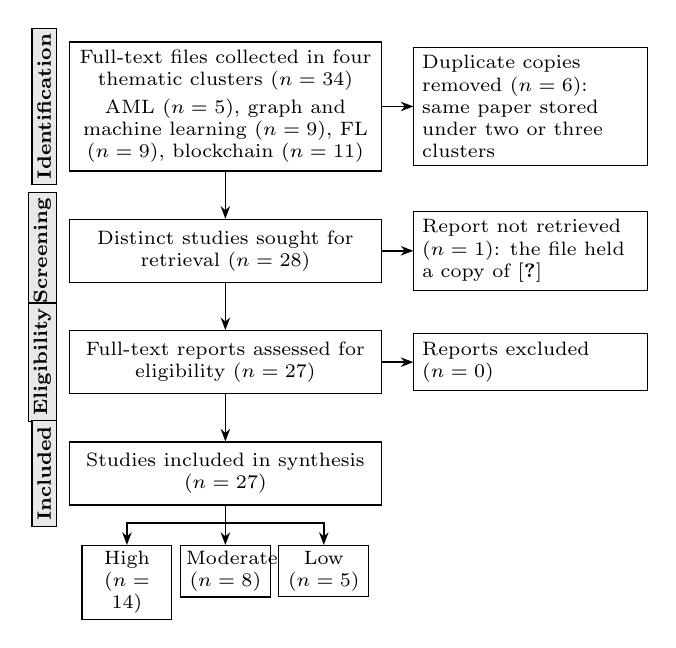
\begin{tikzpicture}[font=\scriptsize,
  box/.style={draw, rectangle, text width=3.75cm, align=flush center, inner sep=3pt, minimum height=8mm},
  side/.style={draw, rectangle, text width=2.75cm, align=flush left, inner sep=3pt},
  small/.style={draw, rectangle, text width=1.0cm, align=flush center, inner sep=2pt},
  arr/.style={-{Stealth[length=1.6mm]}, semithick}]
\node[box] (id) {Full-text files collected in four thematic clusters ($n=34$)\\[2pt] AML ($n=5$), graph and machine learning ($n=9$), FL ($n=9$), blockchain ($n=11$)};
\node[side, right=4mm of id] (dup) {Duplicate copies removed ($n=6$): same paper stored under two or three clusters};
\node[box, below=6mm of id] (sought) {Distinct studies sought for retrieval ($n=28$)};
\node[side, right=4mm of sought] (nr) {Report not retrieved ($n=1$): the file held a copy of \cite{wu2024heists}};
\node[box, below=6mm of sought] (assess) {Full-text reports assessed for eligibility ($n=27$)};
\node[side, right=4mm of assess] (exc) {Reports excluded ($n=0$)};
\node[box, below=6mm of assess] (inc) {Studies included in synthesis ($n=27$)};
\node[small, below=5mm of inc.south, xshift=-1.25cm] (hi) {High\\($n=14$)};
\node[small, below=5mm of inc.south] (mo) {Moderate\\($n=8$)};
\node[small, below=5mm of inc.south, xshift=1.25cm] (lo) {Low\\($n=5$)};
\draw[arr] (id) -- (sought);
\draw[arr] (sought) -- (assess);
\draw[arr] (assess) -- (inc);
\draw[arr] (id) -- (dup);
\draw[arr] (sought) -- (nr);
\draw[arr] (assess) -- (exc);
\draw[arr] (inc.south) -- ++(0,-0.22) -| (hi.north);
\draw[arr] (inc.south) -- (mo.north);
\draw[arr] (inc.south) -- ++(0,-0.22) -| (lo.north);
\foreach \n/\t in {id/Identification, sought/Screening, assess/Eligibility, inc/Included}{
  \node[draw, fill=gray!18, rotate=90, anchor=south, minimum width=8mm, inner sep=2pt, font=\scriptsize\bfseries] at ($(\n.west)+(-1.5mm,0)$) {\t};
}
\end{tikzpicture}
\caption{PRISMA 2020 flow diagram of file collection, deduplication, retrieval, and inclusion.}
\label{fig:prisma}
\end{figure}

Fig.~\ref{fig:prisma} shows the selection process. The four clusters yielded 34 full-text files, 5 on money laundering, 9 on graph and machine learning methods, 9 on FL, and 11 on blockchain. Comparing the files byte by byte, together with their titles and authors, showed that 7 of the 34 files duplicated other files. Six were copies of a paper stored under more than one cluster. The study on CBDC integrity \cite{amber2026cbdc} was stored in three clusters, and the studies by Tang and Liu \cite{tang2024sdt}, Awosika et al. \cite{awosika2024xai}, Ahmed and Alabi \cite{ahmed2024bcfl}, and Ural and Yoshigoe \cite{ural2023bcml} were stored in two clusters each. The seventh file was named after a study on AML customer processes with blockchain and $k$ nearest neighbors, but it contained a copy of the study of Ethereum heists \cite{wu2024heists}. The named study was therefore sought but not retrieved. All 27 distinct reports were assessed in full text. None was excluded under EC2, since the cluster searches were already targeted at the topic, although five studies were graded as low relevance. All 27 studies were included in the synthesis.

\subsection{Data Extraction and Classification}

For each study a structured form recorded the bibliographic data taken from the PDF itself, namely the title, authors, venue, volume, pages, year, and DOI. The form also recorded the problem addressed, the proposed technique, the data and how they were split, the evaluation metrics, the reported results exactly as printed, the threat model where one was stated, and the limitations named by the authors. Where a result appeared only in a figure or in a table stored as an image, the form recorded the relative improvement stated in the text rather than a value read from the image. Each study was assigned one primary category from the seven categories in Table~\ref{tab:taxonomy} and one of three relevance grades. Grade H (high) marks studies that address laundering or fraud detection, or training across institutions for it, with an evaluated technique or a systematic synthesis. Grade M (moderate) marks evaluated techniques or structured surveys from adjacent areas that transfer with adaptation. Grade L (low) marks background, conceptual, or tangential work.

\subsection{Quality Appraisal}

Studies were not excluded on quality grounds. Limitations that affect the weight of their findings were recorded and are reported next to the findings. Nine studies are reviews or surveys and report no new detection experiments \cite{raj2024ai,tiwari2025tbml,li2021befl,dudczyk2024supply,kapadiya2022health,ahmed2024bcfl,ural2023bcml,chen2024finance,jensen2023fighting}. The CBDC framework is evaluated only on synthetic data, and its smart contracts are modeled at the algorithm level rather than deployed on a permissioned chain \cite{amber2026cbdc}. One FL study balances its data with SMOTE before a random split and reports accuracy \cite{awosika2024xai}. MLaD$^2$ assigns accounts to training and test sets at random rather than by time and is evaluated on a single small dataset from one case \cite{luo2024mlad}, and its result tables are available only as images. The labels in GCF-MLD come from analysts reviewing the alerts of a rule system, so they share the blind spots of that system \cite{irshad2024gcfmld}. The FL study of Tang and Liu federates only two clients, each holding a different public dataset \cite{tang2024sdt}. The quantum pipeline evaluates entity resolution on duplicates injected into the data, because Elliptic2 has no ground truth for it, and its authors note that a classical layer of similar size is a relevant baseline for the quantum layer \cite{nayak2026quantum}. Numbers from these studies are reported with the corresponding caveat.

\section{Overview of the Corpus}
\label{sec:corpus}

\begin{table*}[!t]
\centering
\caption{Classification Taxonomy and Distribution of the 27 Reviewed Studies by Relevance (H: High, M: Moderate, L: Low)}
\label{tab:taxonomy}
\footnotesize
\begin{tabularx}{\textwidth}{@{}L{4.6cm}Ycccc@{}}
\toprule
\textbf{Category} & \textbf{Scope} & \textbf{H} & \textbf{M} & \textbf{L} & \textbf{Total}\\
\midrule
AML and TBML reviews & Terminology, stages of laundering, detection practice in banks, TBML literature & 2 & 0 & 1 & 3\\
Graph and machine learning detection & Detectors trained on transaction or account data, graph neural networks, clustering, semi-supervised learning & 6 & 0 & 0 & 6\\
Cryptocurrency and CBDC laundering & Tracing of funds, taint analysis, smart contract enforcement on ledgers & 2 & 0 & 0 & 2\\
FL for financial fraud & Fraud detectors trained across institutions & 3 & 0 & 0 & 3\\
Secure aggregation and attacks on FL & Masking, verification, dropouts, poisoning detection, inference attacks & 0 & 5 & 0 & 5\\
Blockchain for FL and machine learning & Ledgers that coordinate, reward, or secure learning & 1 & 2 & 1 & 4\\
Blockchain for financial records, trade, and documents & Audit trails, trade data, notarization, insurance fraud & 0 & 1 & 3 & 4\\
\midrule
\textbf{Total} & & \textbf{14} & \textbf{8} & \textbf{5} & \textbf{27}\\
\bottomrule
\end{tabularx}
\end{table*}

The corpus is recent. Of the 27 studies, 18 (67\%) were published in 2024 or later, and only three predate 2023 (Fig.~\ref{fig:years}). Journal articles dominate with 23 studies, against four conference papers. IEEE Access alone accounts for 12 studies (Table~\ref{tab:venues}). Three studies appeared in IEEE Transactions on Information Forensics and Security and three in IEEE Transactions on Dependable and Secure Computing. The only study published outside IEEE is the TBML review in the Journal of Accounting Literature \cite{tiwari2025tbml}.

\begin{table}[!t]
\centering
\caption{Venues of the Reviewed Studies (J: Journal, C: Conference)}
\label{tab:venues}
\footnotesize
\begin{tabular}{@{}L{5.6cm}cc@{}}
\toprule
\textbf{Venue} & \textbf{Type} & \textbf{Studies}\\
\midrule
IEEE Access & J & 12\\
IEEE Trans. Information Forensics and Security & J & 3\\
IEEE Trans. Dependable and Secure Computing & J & 3\\
IEEE Trans. Communications & J & 1\\
IEEE Trans. Computational Social Systems & J & 1\\
IEEE Open Journal of the Computer Society & J & 1\\
IEEE Network & J & 1\\
Journal of Accounting Literature (Emerald) & J & 1\\
Int. Joint Conf. Neural Networks (IJCNN) & C & 1\\
Int. Conf. Sentiment Analysis and Deep Learning (ICSADL) & C & 1\\
Int. Conf. Information Technology, Big Data and Artificial Intelligence (ICIBA) & C & 1\\
Int. Conf. Digital Twins and Parallel Intelligence (DTPI) & C & 1\\
\midrule
\textbf{Total} & & \textbf{27}\\
\bottomrule
\end{tabular}
\end{table}

\begin{figure}[!t]
\centering
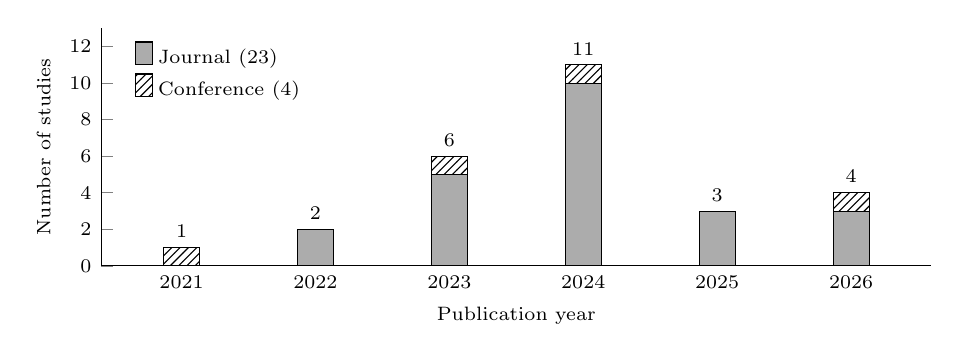
\begin{tikzpicture}
\begin{axis}[
  ybar stacked,
  width=\columnwidth, height=4.6cm,
  bar width=13pt,
  ymin=0, ymax=13,
  ytick={0,2,4,6,8,10,12},
  symbolic x coords={2021,2022,2023,2024,2025,2026},
  xtick=data,
  xlabel={Publication year}, ylabel={Number of studies},
  label style={font=\scriptsize}, tick label style={font=\scriptsize},
  legend style={font=\scriptsize, at={(0.03,0.97)}, anchor=north west, draw=none, fill=none},
  legend cell align=left,
  axis lines*=left,
  enlarge x limits=0.12,
]
\addplot[fill=gray!65, draw=black] coordinates {(2021,0) (2022,2) (2023,5) (2024,10) (2025,3) (2026,3)};
\addplot[fill=white, draw=black, postaction={pattern=north east lines}] coordinates {(2021,1) (2022,0) (2023,1) (2024,1) (2025,0) (2026,1)};
\legend{Journal (23), Conference (4)}
\node[font=\scriptsize, above] at (axis cs:2021,1) {1};
\node[font=\scriptsize, above] at (axis cs:2022,2) {2};
\node[font=\scriptsize, above] at (axis cs:2023,6) {6};
\node[font=\scriptsize, above] at (axis cs:2024,11) {11};
\node[font=\scriptsize, above] at (axis cs:2025,3) {3};
\node[font=\scriptsize, above] at (axis cs:2026,4) {4};
\end{axis}
\end{tikzpicture}
\caption{Publication year of the 27 reviewed studies by venue type.}
\label{fig:years}
\end{figure}

The distribution across categories in Table~\ref{tab:taxonomy} is uneven. Graph and machine learning detection (6 studies) and secure aggregation (5) are the largest categories, while cryptocurrency and CBDC laundering (2) and FL for financial fraud (3) are the smallest. Fourteen studies are graded H, eight M, and five L. The small number of FL studies on financial crime is itself a finding and is discussed in Section~\ref{sec:gaps}.

The application domains are diverse. The corpus covers transfers between bank accounts \cite{irshad2024gcfmld,mao2026pmegnn} and an illegal gambling case \cite{luo2024mlad}. It also covers Bitcoin and Ethereum \cite{ferretti2025gnn,nayak2026quantum,yu2023aetransgat,wu2024heists}, a central bank digital currency \cite{amber2026cbdc}, and fraud with credit cards and bank accounts \cite{tang2024sdt,li2026plc,awosika2024xai}. Studies from adjacent fields address social fintech \cite{xiong2025hppbefl}, health insurance \cite{kapadiya2022health}, IoT networks \cite{yang2022accountable}, supply chains \cite{dudczyk2024supply}, and official documents \cite{cosmin2024notary}. Only one study is about trade-based laundering, and it is a review \cite{tiwari2025tbml}.

\section{RQ1: Detection Models, Data, and Comparability}
\label{sec:rq1}

\begin{figure*}[!t]
\centering
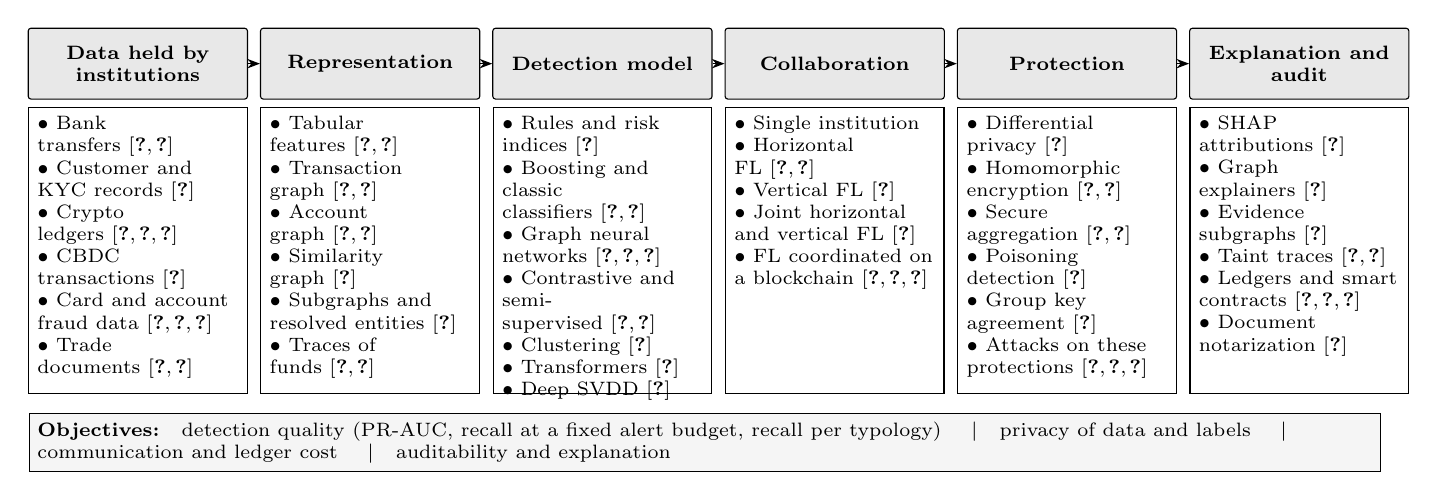
\begin{tikzpicture}[font=\scriptsize,
  head/.style={draw, fill=gray!18, rounded corners=1pt, text width=2.55cm, minimum height=9mm, align=flush center, font=\scriptsize\bfseries},
  body/.style={text width=2.55cm, align=flush left, inner sep=3pt},
  arr/.style={-{Stealth[length=1.6mm]}, semithick}]
\node[head] (h1) at (0,0) {Data held by institutions};
\node[head] (h2) at (2.95,0) {Representation};
\node[head] (h3) at (5.90,0) {Detection model};
\node[head] (h4) at (8.85,0) {Collaboration};
\node[head] (h5) at (11.80,0) {Protection};
\node[head] (h6) at (14.75,0) {Explanation and audit};
\node[body, below=1mm of h1, anchor=north] (b1) {$\bullet$ Bank transfers \cite{irshad2024gcfmld,mao2026pmegnn}\\ $\bullet$ Customer and KYC records \cite{jensen2023fighting}\\ $\bullet$ Crypto ledgers \cite{wu2024heists,ferretti2025gnn,yu2023aetransgat}\\ $\bullet$ CBDC transactions \cite{amber2026cbdc}\\ $\bullet$ Card and account fraud data \cite{tang2024sdt,awosika2024xai,li2026plc}\\ $\bullet$ Trade documents \cite{tiwari2025tbml,dudczyk2024supply}};
\node[body, below=1mm of h2, anchor=north] (b2) {$\bullet$ Tabular features \cite{tang2024sdt,awosika2024xai}\\ $\bullet$ Transaction graph \cite{ferretti2025gnn,yu2023aetransgat}\\ $\bullet$ Account graph \cite{irshad2024gcfmld,mao2026pmegnn}\\ $\bullet$ Similarity graph \cite{luo2024mlad}\\ $\bullet$ Subgraphs and resolved entities \cite{nayak2026quantum}\\ $\bullet$ Traces of funds \cite{amber2026cbdc,wu2024heists}};
\node[body, below=1mm of h3, anchor=north] (b3) {$\bullet$ Rules and risk indices \cite{jensen2023fighting}\\ $\bullet$ Boosting and classic classifiers \cite{amber2026cbdc,mao2026pmegnn}\\ $\bullet$ Graph neural networks \cite{ferretti2025gnn,mao2026pmegnn,yu2023aetransgat}\\ $\bullet$ Contrastive and semi-supervised \cite{luo2024mlad,nayak2026quantum}\\ $\bullet$ Clustering \cite{irshad2024gcfmld}\\ $\bullet$ Transformers \cite{tang2024sdt}\\ $\bullet$ Deep SVDD \cite{li2026plc}};
\node[body, below=1mm of h4, anchor=north] (b4) {$\bullet$ Single institution\\ $\bullet$ Horizontal FL \cite{tang2024sdt,awosika2024xai}\\ $\bullet$ Vertical FL \cite{li2026plc}\\ $\bullet$ Joint horizontal and vertical FL \cite{li2026plc}\\ $\bullet$ FL coordinated on a blockchain \cite{li2021befl,xiong2025hppbefl,ahmed2024bcfl}};
\node[body, below=1mm of h5, anchor=north] (b5) {$\bullet$ Differential privacy \cite{li2026plc}\\ $\bullet$ Homomorphic encryption \cite{yang2022accountable,xiong2025hppbefl}\\ $\bullet$ Secure aggregation \cite{sami2024tinysecagg,wang2023vosa}\\ $\bullet$ Poisoning detection \cite{zhang2023safelearning}\\ $\bullet$ Group key agreement \cite{xiong2025hppbefl}\\ $\bullet$ Attacks on these protections \cite{li2026plc,gao2023category,sami2024tinysecagg}};
\node[body, below=1mm of h6, anchor=north] (b6) {$\bullet$ SHAP attributions \cite{awosika2024xai}\\ $\bullet$ Graph explainers \cite{luo2024mlad}\\ $\bullet$ Evidence subgraphs \cite{nayak2026quantum}\\ $\bullet$ Taint traces \cite{amber2026cbdc,wu2024heists}\\ $\bullet$ Ledgers and smart contracts \cite{amber2026cbdc,chen2024finance,yang2022accountable}\\ $\bullet$ Document notarization \cite{cosmin2024notary}};
\foreach \a/\b in {h1/h2,h2/h3,h3/h4,h4/h5,h5/h6}{\draw[arr] (\a.east) -- (\b.west);}
\coordinate (bot) at ($(b5.south)+(0,-0.08)$);
\foreach \b in {b1,b2,b3,b4,b5,b6}{\draw (\b.north west) rectangle (\b.east |- bot);}
\node[draw, fill=gray!8, anchor=north west, text width=16.95cm, align=flush left, inner sep=3pt] (obj) at ($(b1.west |- bot)+(0,-0.25)$) {\textbf{Objectives:}\quad detection quality (PR-AUC, recall at a fixed alert budget, recall per typology) \quad$\mid$\quad privacy of data and labels \quad$\mid$\quad communication and ledger cost \quad$\mid$\quad auditability and explanation};
\end{tikzpicture}
\caption{Pipeline of techniques for detecting laundering across institutions as studied in the reviewed literature. Each stage lists the options that primary studies evaluate or propose. Together they determine the objectives in the bottom row.}
\label{fig:taxonomy}
\end{figure*}

Fig.~\ref{fig:taxonomy} places the techniques of the corpus in one pipeline, from the data each institution holds to the audit of the alerts it produces. This section covers the representation of the data and the detection model. Table~\ref{tab:detection} summarizes the detection studies.

\subsection{From Rules to Learned Detectors}

Rules remain the baseline against which learned detectors are measured. In the bank studied by Irshad et al., every account in the data had already triggered an alert in the rule system of the bank, and analysts had escalated 75 of the 9{,}925 alerted accounts as SARs \cite{irshad2024gcfmld}. Jensen and Iosifidis find that published work on flagging relies on undisclosed features and risk indices built by hand, which makes the methods hard to reuse \cite{jensen2023fighting}. Classic classifiers still appear. In the CBDC framework, a random forest and a support vector machine reach accuracies of 91.11\% and 93.12\% on two synthetic scenarios \cite{amber2026cbdc}. Gradient boosting remains a strong baseline. On the IBM HI-Small data, XGBoost and LightGBM with graph features reach a minority class F1 of 63.23 and 62.86, ahead of several graph neural networks \cite{mao2026pmegnn}.

\subsection{Graph Representations}

Most of the corpus treats laundering as a property of a network rather than of a single transfer. Three graph designs appear. In a transaction graph, nodes are transactions and edges are flows of funds between them, as in the Elliptic data \cite{ferretti2025gnn,yu2023aetransgat}. In an account graph, nodes are accounts and edges are transfers \cite{irshad2024gcfmld,mao2026pmegnn}. MLaD$^2$ builds a third kind, a weighted graph in which the weight of an edge reflects how similar two accounts are, computed from 32 behavior statistics over daily time slices \cite{luo2024mlad}. The reason is that laundering accounts trade with benign accounts on purpose to hide, so a model that assumes neighbors are alike mixes the two classes \cite{luo2024mlad}.

Features matter as much as structure. Ferretti et al. removed the features supplied with Elliptic and kept only the graph and node metrics, and the results became very poor \cite{ferretti2025gnn}. Adding features aggregated from neighboring transactions to the features of the transaction itself improved graph networks \cite{ferretti2025gnn}, and it also improved logistic regression, multilayer perceptrons, and support vector machines \cite{yu2023aetransgat}.

\begin{table*}[!t]
\centering
\caption{Detection Studies and Their Results as Reported. Numbers Are Not Comparable Across Rows Because Data, Splits, and Metrics Differ}
\label{tab:detection}
\footnotesize
\begin{tabularx}{\textwidth}{@{}L{1.9cm}L{3.1cm}L{2.35cm}YL{1.75cm}L{3.3cm}@{}}
\toprule
\textbf{Study} & \textbf{Data} & \textbf{Split} & \textbf{Model} & \textbf{Metric} & \textbf{Reported result}\\
\midrule
AEtransGAT \cite{yu2023aetransgat} & Elliptic, Bitcoin transactions & 70/30 by time & Graph attention weighted by amount, graph autoencoder, mutual learning & F1 & 0.899 (GAT 0.838, GCN 0.759)\\
Ferretti et al. \cite{ferretti2025gnn} & Elliptic, Bitcoin transactions & Not stated, repeated runs & Chebyshev convolutions with a final linear layer & Illicit class F1 & 0.906 (GCN at most 0.667)\\
Quantum-Enhanced AML \cite{nayak2026quantum} & Elliptic2 subgraphs of Bitcoin clusters & Chronological, repeated runs & GNN with quantum layer, entity resolution, temporal contrastive learning & F1, AUC & 0.969, 0.995\\
PME-GNN \cite{mao2026pmegnn} & IBM HI-Small and LI-Small & 60/20/20 by time, five seeds & Principal neighbourhood aggregation with positional encoding and sparse experts & Minority class F1 (\%) & $74.81\pm1.23$ (HI), $38.23\pm2.14$ (LI)\\
MLaD$^2$ \cite{luo2024mlad} & Illegal gambling case, 51{,}326 transactions & Random by account, 70/10/20, ten repetitions & GNN on similarity graph with contrastive pretraining & F1 gain & $+2.71\%$ over XGBoost, $+24.80\%$ over unsupervised baselines with 10\% labels\\
GCF-MLD \cite{irshad2024gcfmld} & One bank, 1.771 million transactions, 75 SAR accounts & No training labels & Graph features with hierarchical clustering & Precision, recall, AUC & 87.32\%, 82.67\%, 0.91\\
CBDC framework \cite{amber2026cbdc} & Two synthetic scenarios & Not stated & Random forest and support vector machine with taint analysis & Accuracy & 91.11\%, 93.12\%\\
\bottomrule
\end{tabularx}
\end{table*}

\subsection{Graph Neural Networks}

On Elliptic, AEtransGAT weights each neighbor by the amount transferred and trains a graph autoencoder alongside the classifier, so that the model also learns to reconstruct the structure of the graph. It reaches an F1 of 0.899, against 0.838 for a plain graph attention network and 0.759 for a graph convolutional network \cite{yu2023aetransgat}. Ferretti et al. reach an illicit class F1 of 0.906 with Chebyshev convolutions, a final linear layer, and a reduced set of aggregated features, while their graph convolutional networks stay at or below 0.667 \cite{ferretti2025gnn}. Unsupervised graph anomaly detectors reach only 0.62 to 0.68 on the same data \cite{yu2023aetransgat}, which shows how much the labels contribute.

On the IBM HI-Small data, PME-GNN extends principal neighbourhood aggregation with positional encodings from random walks, message passing in both directions of each payment, attention over features, and a sparse mixture of experts. It reaches a minority class F1 of $74.81\pm1.23$ over five seeds, against 56.77 for principal neighbourhood aggregation alone \cite{mao2026pmegnn}. Its baselines include the variants of graph isomorphism networks that Egressy et al. proposed for directed multigraphs \cite{egressy2024multignn}. On the LI-Small subset, where laundering is about half as frequent, the same model reaches only $38.23\pm2.14$ \cite{mao2026pmegnn}. The base rate matters as much as the architecture.

Two studies reduce the dependence on labels. MLaD$^2$ pretrains on unlabeled accounts with contrastive learning and then trains on the labels. With labels for only 10\% of the training accounts it improves F1 by 24.80\% over the best unsupervised baseline, and it improves on XGBoost by 2.71\% \cite{luo2024mlad}. It keeps a false positive rate of zero in all reported comparisons and trains on 51{,}326 transactions in under four minutes \cite{luo2024mlad}. The Quantum-Enhanced AML pipeline merges duplicate entities before learning, adds contrastive learning across time windows, and passes a pooled summary of each subgraph through a parameterized quantum circuit \cite{nayak2026quantum}. On Elliptic2 it reports an F1 of up to 0.969 and an AUC of up to 0.995, and removing entity resolution lowers them to 0.954 and 0.989 \cite{nayak2026quantum}. The authors note that a classical layer with a similar number of parameters could recover part of the gain attributed to the quantum layer \cite{nayak2026quantum}.

GCF-MLD takes an unsupervised route on real bank data. It adds centrality and connectivity measures from the account graph to account and transaction features and flags the outliers of K-means and hierarchical clustering \cite{irshad2024gcfmld}. Against the SAR labels, hierarchical clustering reaches a precision of 87.32\%, a recall of 82.67\%, and an AUC of 0.91, while K-means reaches 84.12\%, 70.67\%, and 0.85 \cite{irshad2024gcfmld}.

\subsection{Comparability of Reported Results}
\label{sec:comparability}

Table~\ref{tab:detection} collects the results as published, and they cannot be ranked against each other. The studies use five different data sources, and even on Elliptic they report different variants of F1. The splits differ as well. PME-GNN uses a 60/20/20 split by time \cite{mao2026pmegnn}, AEtransGAT a 70/30 split by time \cite{yu2023aetransgat}, and the quantum pipeline a chronological split \cite{nayak2026quantum}. MLaD$^2$ assigns accounts to training and test sets at random \cite{luo2024mlad}, so its model is trained on a network observed over the same period in which it is tested. PME-GNN \cite{mao2026pmegnn}, Ferretti et al. \cite{ferretti2025gnn}, and the quantum pipeline \cite{nayak2026quantum} report means and standard deviations over repeated runs, MLaD$^2$ averages ten repetitions \cite{luo2024mlad}, and the remaining detection studies report a single value.

The metrics differ most. Jensen and Iosifidis advise strongly against accuracy for AML because of the extreme class imbalance \cite{jensen2023fighting}, and PME-GNN shows that a model that labels every transfer as legitimate scores about 99.9\% accuracy on HI-Small \cite{mao2026pmegnn}. Two studies in the corpus still report accuracy as their main result \cite{amber2026cbdc,awosika2024xai}. Only one study reports the area under the precision recall curve \cite{tang2024sdt}, the measure that Jensen and Iosifidis recommend when imbalance is severe \cite{jensen2023fighting}.

\subsection{Cryptocurrency Flows and Taint Analysis}

Two studies trace funds rather than classify them. XBlockFlow starts from the accounts behind 73 Ethereum security incidents between 2016 and 2022 and follows the stolen funds layer by layer until they reach service providers such as exchanges \cite{wu2024heists}. The resulting EthereumHeist dataset labels more than 160{,}000 addresses with their layer and the kind of service at the exit, which the binary labels of Elliptic cannot express \cite{wu2024heists}. It documents methods that do not exist in Bitcoin, such as token swaps, counterfeit tokens, and posing as speculators \cite{wu2024heists}. Amber et al. combine taint analysis with smart contracts and classifiers for a CBDC and report an average tracking time of 0.55~s \cite{amber2026cbdc}. Tracing of this kind needs a ledger that the analyst can read, so it does not apply directly to bank transfers that each bank keeps to itself.

\subsection{Synthesis}

The evidence on detection agrees in direction even though the numbers cannot be compared. Structure helps. Features aggregated from neighboring transactions improve every model family tested on Elliptic \cite{ferretti2025gnn,yu2023aetransgat}, and following payments in both directions improves results on the IBM data \cite{mao2026pmegnn}. Structure alone is not enough, since the graph without the supplied features performs poorly and unsupervised detectors trail those trained on labels \cite{ferretti2025gnn,yu2023aetransgat}. The rarity of laundering sets a ceiling that the model alone cannot lift, as the gap between HI-Small and LI-Small shows \cite{mao2026pmegnn}. Every detection study in the corpus trains on data held in one place, and only the quantum pipeline names collaboration across institutions, as future work \cite{nayak2026quantum}.

\section{RQ2: Federated Learning for Fraud and Laundering Detection}
\label{sec:rq2}

Three studies train fraud detectors across institutions with FL \cite{tang2024sdt,awosika2024xai,li2026plc}. None of them uses laundering data. Table~\ref{tab:fl} compares their settings.

\begin{table*}[!t]
\centering
\caption{Federated Learning Studies on Financial Fraud}
\label{tab:fl}
\footnotesize
\begin{tabularx}{\textwidth}{@{}L{1.75cm}L{2.1cm}L{1.85cm}L{3.3cm}YL{1.9cm}L{3.0cm}@{}}
\toprule
\textbf{Study} & \textbf{Setting} & \textbf{Clients} & \textbf{Data} & \textbf{Different data across clients} & \textbf{Protection} & \textbf{Reported result}\\
\midrule
Tang and Liu \cite{tang2024sdt} & Horizontal, structured data transformer & Two simulated banks & European card data (284{,}807, 0.172\% fraud) and simulated card data (1{,}296{,}675, 0.579\% fraud) & Each bank has its own linear input layer before the shared model & None stated & Federated AUC-PR 0.884 and 0.892 against 0.882 and 0.816 when trained alone\\
Awosika et al. \cite{awosika2024xai} & Horizontal, dense network & Three, random split of one dataset & 29{,}042 bank account records, balanced with SMOTE & None, clients share one distribution & None, SHAP for explanation & Accuracy 93\%\\
PLC \cite{li2026plc} & Joint horizontal and vertical & Two groups of ten clients, four committee members & European card data and Vesta (590{,}540, 394 features, 3.17\% fraud) & Vertical groups hold different features for matched customers & Sparse secure multiparty aggregation & Communication 46.7\% and 55.4\% lower than ELSA, F1 14.4\% and 46.4\% above anomaly detectors\\
\bottomrule
\end{tabularx}
\end{table*}

\subsection{Horizontal Federation of Banks}

Awosika et al. split one dataset of 29{,}042 bank account records from the Bank Account Fraud suite \cite{jesus2022baf} at random among three clients, train a small dense network, and explain its predictions with SHAP \cite{awosika2024xai}. The data were balanced with SMOTE before the split, and the model reaches an accuracy of 93\% \cite{awosika2024xai}. Because the clients share one distribution and the test set is balanced, the setting says little about banks whose customers and fraud rates differ.

Tang and Liu federate two simulated banks that hold different public credit card datasets \cite{tang2024sdt}. Each bank trains a structured data transformer, the server aggregates the parameters, and each bank then blends the global parameters into its local model through a momentum update \cite{tang2024sdt}. Federation raised the area under the precision recall curve on the second dataset from 0.816 to 0.892 and its F1 from 0.754 to 0.822, and it left the first dataset almost unchanged at 0.884 against 0.882 \cite{tang2024sdt}.

\subsection{Institutions With Different Data}

Banks do not hold the same columns. Tang and Liu are the only study in the corpus that federates clients with different feature spaces without matching their customers. Each bank passes its data through its own linear layer, which maps it to a common size before the shared transformer \cite{tang2024sdt}. With two clients and two public datasets the design is a proof of concept, but it is the closest precedent for banks that keep their own schemas.

PLC by Li et al. combines horizontal and vertical FL for an alliance across industries \cite{li2026plc}. Within a group, such as several banks, the members hold the same features for different customers and train a model of normal behavior with Deep SVDD on all their local data. Across groups, such as a bank, an online shop, and a regulator, the members hold different features for the same customers and train the fraud detector with secure multiparty computation \cite{li2026plc}. The horizontal stage uses the records that private set intersection would otherwise discard \cite{li2026plc}. The authors state two assumptions, that data within a group are independent and identically distributed and that features align across groups, and they name heterogeneity across industries as the main open problem \cite{li2026plc}.

Two kinds of heterogeneity matter for laundering, and neither is tested in the corpus. The first is the schema, since each bank computes different features from account history and stores different customer attributes. The second is the skew of labels, since the share of laundering can differ greatly between banks and some banks may hold no confirmed cases at all.

\subsection{Communication and Cost}

Communication is the other practical constraint. The sparse aggregation of PLC cuts communication by 46.7\% on the European card data and by 55.4\% on the larger Vesta data compared with ELSA, and on Vesta its F1 is 7.3\% higher on average than that of differential privacy with a privacy budget of 0.1 \cite{li2026plc}. TinySecAgg reduces the communication of secure aggregation by up to 22.5 times through sparsification \cite{sami2024tinysecagg}, as discussed in Section~\ref{sec:rq3}. No study reports the communication cost of FL on laundering data.

\section{RQ3: Secure Aggregation and Its Limits}
\label{sec:rq3}

Five studies design or attack secure aggregation \cite{yang2022accountable,zhang2023safelearning,gao2023category,sami2024tinysecagg,wang2023vosa}, and two more use cryptographic aggregation inside larger systems \cite{xiong2025hppbefl,li2026plc}. Table~\ref{tab:sa} compares them.

\begin{table*}[!t]
\centering
\caption{Secure Aggregation Schemes and Attacks in the Corpus}
\label{tab:sa}
\footnotesize
\begin{tabularx}{\textwidth}{@{}L{2.2cm}YL{3.6cm}L{3.9cm}@{}}
\toprule
\textbf{Scheme} & \textbf{Mechanism} & \textbf{Adds to basic secure aggregation} & \textbf{Evaluation}\\
\midrule
VOSA \cite{wang2023vosa} & Aggregator-oblivious encryption with dynamic group management & Users can verify the aggregate, tolerance to dropouts & MNIST with a multilayer perceptron and a CNN\\
Yang et al. \cite{yang2022accountable} & Homomorphic proxy primitives for authentication and encryption, deposits on a blockchain & Verifiable origin of contributions, penalties for misbehaving clients, flexible dropouts & Ethereum prototype with ten clients\\
SAFELearning \cite{zhang2023safelearning} & Oblivious random subgroups with partial disclosure of subgroup aggregates & Backdoor detection while individual updates stay hidden & ResNet-18 on CIFAR-10\\
TinySecAgg \cite{sami2024tinysecagg} & Masking of sparsified gradients that also hides their coordinates & Up to 22.5 times less communication without loss of accuracy & Formal privacy guarantees and experiments\\
HPP-BEFL \cite{xiong2025hppbefl} & Group key agreement across public key and identity-based systems & Aggregation of encrypted models among participants with different cryptosystems & Security proofs and efficiency experiments\\
PLC \cite{li2026plc} & Sparse secure multiparty aggregation with a committee & Lower communication, resistance to gradient inversion and inference attacks & European card data and Vesta\\
Category inference \cite{gao2023category} & Attack on secure aggregation with differential selection and denoising & Shows which classes each client holds & F1 above 90\% in most cases on MNIST, CIFAR-10, AG\_news, and DBPedia\\
\bottomrule
\end{tabularx}
\end{table*}

\subsection{What Secure Aggregation Protects}

Secure aggregation lets the server learn the sum of the updates and nothing about any single update \cite{bonawitz2017secagg}. In the original protocol each pair of users agrees on random masks that cancel when the masked updates are added \cite{sami2024tinysecagg}. The corpus extends this guarantee in three directions. VOSA lets users check that the server did not forge the aggregate, which matters when the server skips part of the work to save resources or acts maliciously, and it keeps working when users drop out \cite{wang2023vosa}. The scheme of Yang et al. lets the origin of each contribution be verified and uses a blockchain to hold deposits and to penalize clients that misbehave \cite{yang2022accountable}. HPP-BEFL lets participants that use different public key systems agree on a group key, so that the server can aggregate encrypted models without decrypting them \cite{xiong2025hppbefl}.

\subsection{What It Does Not Protect}

Hiding individual updates is not the same as hiding what the data contain. Gao et al. define category privacy as the set of classes a client holds and show that secure aggregation does not protect it when the data of the clients are not identically distributed \cite{gao2023category}. Their attack infers the categories of each client with an F1 above 90\% in most cases on four image and text datasets \cite{gao2023category}. In a federation of banks the positive class is laundering. Whether a bank holds confirmed laundering accounts is sensitive information about its customers and its compliance record, and this result suggests that secure aggregation alone would not hide it. No AML study in the corpus measures this leakage.

Optimizing for cost can open new channels. When gradients are sparsified before secure aggregation, the indices of the coordinates that each user sends leak information about its data, even though the values stay hidden \cite{sami2024tinysecagg}. TinySecAgg hides the coordinates as well and still reduces communication by up to 22.5 times compared with conventional secure aggregation, without loss of accuracy \cite{sami2024tinysecagg}.

\subsection{Poisoning Under Encryption}

Encryption also makes poisoning easier to hide, because anomaly detectors usually need to see each update in the clear \cite{zhang2023safelearning}. SAFELearning assigns users to random subgroups that no user can learn and discloses only the aggregate of each subgroup, whose statistics reveal backdoors \cite{zhang2023safelearning}. With ResNet-18 on CIFAR-10 it reduces backdoor accuracy to zero in most cases when attackers are few, and training converges at a rate similar to plain FL \cite{zhang2023safelearning}. Yang et al. take a different route and penalize misbehavior after the fact through deposits held on a blockchain \cite{yang2022accountable}. None of these defenses has been tested with a financial model, where a poisoned update could teach the global model to ignore a laundering pattern.

\subsection{Synthesis}

The protections in the corpus were evaluated on images, text, and IoT data \cite{yang2022accountable,zhang2023safelearning,gao2023category,sami2024tinysecagg,wang2023vosa}. The financial FL studies use either no cryptographic protection \cite{tang2024sdt,awosika2024xai} or protection against servers that follow the protocol but try to learn from what they receive \cite{li2026plc}. A federation of banks needs secure aggregation that can verify the aggregate, detect poisoning, tolerate dropouts, and hide which banks hold laundering cases. Each property exists in some scheme, but no scheme combines them.

\section{RQ4: Blockchain for Auditable Learning and Records}
\label{sec:rq4}

\subsection{Roles of the Ledger}

\begin{table}[!t]
\centering
\caption{Roles of Blockchain in the Corpus}
\label{tab:blockchain}
\footnotesize
\begin{tabular}{@{}L{1.85cm}L{3.55cm}L{2.1cm}@{}}
\toprule
\textbf{Role} & \textbf{What the ledger holds} & \textbf{Studies}\\
\midrule
Coordinating FL & Updates and agreement on the aggregate, replacing the single server & \cite{li2021befl,xiong2025hppbefl,ahmed2024bcfl}\\
Incentives and marketplaces & Contributions of data and models and their rewards & \cite{li2021befl,ural2023bcml}\\
Accountability & Deposits, tracing challenges, and penalties & \cite{yang2022accountable}\\
Policy enforcement & Transaction validation and AML rules in smart contracts & \cite{amber2026cbdc}\\
Integrity of records & Transactions, document hashes, and access logs as an audit trail & \cite{dudczyk2024supply,kapadiya2022health,cosmin2024notary,chen2024finance}\\
\bottomrule
\end{tabular}
\end{table}

Blockchain plays five roles in the corpus, summarized in Table~\ref{tab:blockchain}. The first is to replace the central FL server. Li et al. describe a framework of six layers for FL on a blockchain, from infrastructure and consensus through incentives, smart contracts, and privacy protection up to applications. They argue that a ledger removes the single point of failure of the server and lets participants check the quality of updates \cite{li2021befl}. The second is to reward the sharing of data and models through incentives and marketplaces \cite{li2021befl,ural2023bcml}. The third is accountability. Yang et al. record deposits, tracing challenges, and penalties on Ethereum, so that a client caught misbehaving loses its deposit \cite{yang2022accountable}. The fourth is policy enforcement. In the CBDC framework, smart contracts validate transactions and enforce AML rules \cite{amber2026cbdc}. The fifth is the integrity of records. Chen et al. describe the ledger as a consistent audit trail that regulators can follow to trace funds, and smart contracts as a way to share identity information for compliance while keeping it private \cite{chen2024finance}. Cosmin-Iulian and Adrian hash an official document, obfuscate its sensitive fields, hash it again, and keep both hashes in storage built on IPFS and a private Ethereum network, so that the document can be shared in part and still be verified \cite{cosmin2024notary}.

\subsection{Cost and Scale}

The ledger has a cost. In the prototype of Yang et al., a deposit transaction costs 144{,}529 gas and a penalty transaction 357{,}626 gas on Ethereum \cite{yang2022accountable}. Ahmed and Alabi identify scalability as the main obstacle for FL built on blockchain in fraud detection. They point to light consensus protocols such as proof of authority, whose complexity grows linearly with the number of validators, and they note that adding differential privacy or secure multiparty computation raises the overhead further \cite{ahmed2024bcfl}. Amber et al. could not deploy their smart contracts on a permissioned chain and modeled them at the algorithm level instead \cite{amber2026cbdc}.

\subsection{What Is Recorded and What Is Not}

No study records the life cycle of a laundering detector on a ledger, from the update that each bank sends, through the aggregated model of each round, to the alerts that the model raises and the reasons it gives for them. The ledgers in the corpus hold deposits and penalties \cite{yang2022accountable}, policies \cite{amber2026cbdc}, or documents \cite{cosmin2024notary,chen2024finance}. Writing hashes rather than data keeps the ledger small and keeps customer data off it. This approach is used for documents \cite{cosmin2024notary} but not yet for models and alerts.

The supply chain literature is relevant for TBML. Dudczyk et al. list blockchain platforms for global trade, such as TradeLens by IBM and Maersk and the BDTS of CargoX, and cite work that names customs programs driven by data and the detection of financial crime among the uses of blockchain in trade \cite{dudczyk2024supply}. A ledger of trade documents could give a detector verified invoices and shipping records to match against payments.

\section{RQ5: Explaining Alerts to Analysts and Auditors}
\label{sec:rq5}

An alert must be explained before an analyst can act on it, and regulated institutions must be able to justify their models later \cite{jensen2023fighting,chen2024finance}. The corpus uses four kinds of explanation, compared in Table~\ref{tab:xai}.

\begin{table}[!t]
\centering
\caption{Explanations Produced by the Reviewed Studies}
\label{tab:xai}
\footnotesize
\begin{tabular}{@{}L{1.25cm}L{2.0cm}L{1.75cm}L{1.05cm}L{1.0cm}@{}}
\toprule
\textbf{Study} & \textbf{Explanation} & \textbf{Unit} & \textbf{Assessed by users} & \textbf{Tied to model version}\\
\midrule
\cite{awosika2024xai} & SHAP plots for two clients & Features & No & No\\
\cite{luo2024mlad} & PGM-Explainer and most similar neighbors & Neighbor accounts & No & No\\
\cite{nayak2026quantum} & Evidence subgraph per flagged case & Paths and neighbors & No & No\\
\cite{wu2024heists} & Taint trace from a known incident & Chains of addresses & No & No\\
\cite{amber2026cbdc} & Taint analysis, SHAP and LIME planned & Flows of funds & No & No\\
\bottomrule
\end{tabular}
\end{table}

\subsection{Feature Attribution}

Awosika et al. explain their federated model with SHAP \cite{lundberg2017shap} and show attribution plots for two clients \cite{awosika2024xai}. SHAP gives each feature its average marginal contribution over all subsets of the other features \cite{lundberg2017shap}, and it works with any model and with tabular bank features. The plots in that study label the features by their values rather than their names, and no analyst evaluates them \cite{awosika2024xai}. Amber et al. list SHAP and LIME as future work for their CBDC framework \cite{amber2026cbdc}, and Jensen and Iosifidis name interpretable and fair machine learning among the main open directions for AML \cite{jensen2023fighting}.

\subsection{Graph Explanations and Evidence Subgraphs}

Graph models need explanations in terms of accounts and paths. MLaD$^2$ uses PGM-Explainer to highlight the neighbors that decided the class of an account and lists the five most similar neighbors with their cosine similarities \cite{luo2024mlad}. Its authors still describe the inherent interpretability of the model as weak \cite{luo2024mlad}. The quantum pipeline extracts an evidence subgraph for every flagged case, with the key paths and neighbors behind the risk score, as material for review by an analyst \cite{nayak2026quantum}. It measures how faithful and how stable these subgraphs are, but not how useful analysts find them \cite{nayak2026quantum}.

\subsection{Traces of Funds}

Tracing studies explain by construction, since each flagged address comes with the chain of transfers that links it to a known incident \cite{wu2024heists} or to tainted funds \cite{amber2026cbdc}. This kind of explanation is easy for an investigator to check, but it depends on a ledger that the investigator can read.

\subsection{Explanations as Audit Records}

An explanation is useful later only if it can be tied to the model and the data that produced it. None of the studies stores its explanations with a reference to the model version, and none keeps them in a form that would show later changes. Section~\ref{sec:arch} proposes binding each alert, its score, its main attributions, and the model version into one hash that is written to the ledger.

\section{RQ6: Trade-Based Money Laundering}
\label{sec:rq6}

\subsection{What the TBML Literature Offers}

Tiwari et al. searched Scopus and Web of Science in October 2022 for peer-reviewed journal articles published since the FATF report of 2006 \cite{tiwari2025tbml}. After removing duplicates they had 33 records, and they added 214 candidate records found by citation mapping, which they then sampled purposively \cite{tiwari2025tbml}. They sort the literature into four themes, namely risk assessment, detection, the role of professionals, and understanding of the crime \cite{tiwari2025tbml}.

Detection methods fall into two groups \cite{tiwari2025tbml}. Statistical methods compare the declared price of goods with average prices to find outliers, in the line of the work of Zdanowicz on abnormal trade prices \cite{zdanowicz2009}. Economic methods treat laundering as the dependent variable of a regression on prices and payments. Trade gap or mirror analysis, which compares what one country reports exporting with what its partner reports importing, has been applied to Italian trade data \cite{tiwari2025tbml}. A single study applies a classification algorithm to data from Chinese provinces, without comparing it with other methods \cite{tiwari2025tbml}.

\subsection{Limits of Current TBML Detection}

These methods mainly detect mispriced invoices and miss other forms of TBML \cite{tiwari2025tbml}. They need detailed trade data of high quality, which are often unavailable. They also ignore context such as the nature of the goods and the relationship between the parties, which produces false positives \cite{tiwari2025tbml}. One method assumes that goods are declared at the same value in the exporting and the importing country and so ignores freight, insurance, tariffs, and exchange rates \cite{tiwari2025tbml}. Tiwari et al. conclude that the literature is too thin to say how TBML is best fought, and they call for work on its definition, its typologies, the weaknesses it exploits, and the response of practitioners \cite{tiwari2025tbml}. They also note that TBML can occur without manipulating price or quantity, and through payment methods other than cash and banks \cite{tiwari2025tbml}.

\subsection{What Transfers From Transaction Monitoring}

No study in the corpus applies graph learning, FL, or blockchain auditing to TBML. Several techniques nonetheless transfer. Trade involves the same parties that appear in payment networks, so graph features and graph models built on counterparties \cite{irshad2024gcfmld,mao2026pmegnn} can be extended to networks of importers, exporters, and shippers. Vertical FL suits TBML better than horizontal FL, because a bank, a customs authority, and a shipping line hold different facts about the same trade \cite{li2026plc}. The joint scheme of PLC shows how organizations from different fields can train together without discarding records that cannot be matched \cite{li2026plc}. Ledgers of trade documents \cite{dudczyk2024supply} and verified partial disclosure of documents \cite{cosmin2024notary} can supply the trusted invoice and shipment records that price analysis needs. Synthetic data, recommended for transaction AML \cite{ferretti2025gnn,jensen2023fighting} and used to build the IBM benchmark \cite{altman2023ibmaml}, has no counterpart for trade in the corpus, so a simulator of trade with injected mispricing would be a natural first step.

\section{Research Gaps and Open Challenges}
\label{sec:gaps}

\begin{table*}[!t]
\centering
\caption{Open Research Gaps With Supporting Evidence and the Closest Existing Work}
\label{tab:gaps}
\footnotesize
\begin{tabularx}{\textwidth}{@{}L{3.55cm}YL{2.4cm}L{4.4cm}@{}}
\toprule
\textbf{Gap} & \textbf{Evidence in the corpus} & \textbf{Closest work} & \textbf{Opportunity}\\
\midrule
G1 FL on laundering data & Three FL studies, all on card or account fraud & \cite{tang2024sdt,awosika2024xai,li2026plc} & FL across banks on the IBM data\\
G2 Banks with different schemas & Input layers per bank with two clients, joint FL that assumes aligned features & \cite{tang2024sdt,li2026plc} & Shared core encoder with private encoders per bank\\
G3 Comparable evaluation & Accuracy on balanced data, random splits, few seeds, PR-AUC reported once & \cite{jensen2023fighting,mao2026pmegnn} & Splits by time, PR-AUC, recall per typology, several seeds\\
G4 Category privacy & Secure aggregation reveals which classes a client holds & \cite{gao2023category} & Measuring and bounding the leakage of laundering presence\\
G5 Verifiable aggregation that resists poisoning & Verification, poisoning detection, and dropouts solved separately on images & \cite{yang2022accountable,zhang2023safelearning,wang2023vosa} & One protocol tested on financial models\\
G6 Auditable model life cycle & Ledgers hold deposits, policies, or documents & \cite{amber2026cbdc,yang2022accountable,cosmin2024notary} & Hashes of updates, models, and alerts on a permissioned chain\\
G7 Explanations as evidence & SHAP plots not assessed, graph explanations weak & \cite{awosika2024xai,luo2024mlad,nayak2026quantum} & Explanations tied to model versions and assessed with analysts\\
G8 Scarce labels and drift & Labels late and partly subjective, periodic retraining & \cite{irshad2024gcfmld,luo2024mlad,nayak2026quantum} & Semi-supervised and temporal training in a federation\\
G9 Public and documented data & Elliptic undocumented, bank data private, no trade data & \cite{ferretti2025gnn,altman2023ibmaml} & Documented synthetic data with customers and trade\\
G10 Detection of TBML & Price statistics, mirror analysis, one classifier & \cite{tiwari2025tbml,zdanowicz2009} & Vertical federation of bank, customs, and shipping data\\
\bottomrule
\end{tabularx}
\end{table*}

Table~\ref{tab:gaps} summarizes ten gaps that emerge from the synthesis together with the closest existing work. The first five concern learning across institutions and its protection.

\textbf{G1. FL on laundering data.} The three FL studies detect card or account fraud \cite{tang2024sdt,awosika2024xai,li2026plc}. None trains across banks on laundering data, although the IBM transactions record the sending and receiving bank of every transfer and can therefore be divided among simulated banks \cite{altman2023ibmaml,mao2026pmegnn}. Results on fraud do not carry over directly, since laundering is rarer, unfolds in patterns of many steps, and is spread across institutions on purpose.

\textbf{G2. Banks with different schemas.} Banks compute different features from account history and keep different customer attributes. Input layers per bank handle this for two clients \cite{tang2024sdt}, and joint FL handles different features only for customers matched across groups \cite{li2026plc}. A design in which banks share an encoder for the fields every bank has, keep private encoders for their own fields, and share the prediction head has not been evaluated in the corpus.

\textbf{G3. Comparable evaluation.} The studies differ in data, splits, metrics, and repetitions (Section~\ref{sec:comparability}). A shared protocol would fix a split by time, report the area under the precision recall curve together with recall at a fixed alert budget, give recall for each laundering typology, and average over seeds. The quantum pipeline already reports results under fixed alert budgets \cite{nayak2026quantum}, which match how analysts work through a queue.

\textbf{G4. Category privacy.} Secure aggregation leaks which classes a client holds \cite{gao2023category}. In AML this means which banks hold confirmed laundering cases. The leakage has not been measured for any financial federation, and the corpus does not discuss defenses against it.

\textbf{G5. Verifiable aggregation that resists poisoning.} Verification of the aggregate \cite{wang2023vosa}, detection of backdoors \cite{zhang2023safelearning}, tolerance to dropouts \cite{wang2023vosa}, and accountability \cite{yang2022accountable} exist in separate schemes, all evaluated on images or IoT data. A federation of banks needs them together, with a model small enough to keep the cryptography cheap.

The remaining five concern auditability, labels, data, and trade.

\textbf{G6. Auditable model life cycle.} The ledgers in the corpus record deposits and penalties \cite{yang2022accountable}, AML policies \cite{amber2026cbdc}, and documents \cite{cosmin2024notary}. None records which update each bank sent, which model each round produced, and which model raised each alert. Without that record an auditor cannot check later that an alert came from an approved model.

\textbf{G7. Explanations as evidence.} SHAP plots are shown without assessment \cite{awosika2024xai}, graph explanations are produced after the fact and are weak by the account of their own authors \cite{luo2024mlad}, and evidence subgraphs are measured for fidelity and stability but not assessed with analysts \cite{nayak2026quantum}. No study ties an explanation to the model version that produced it.

\textbf{G8. Scarce labels and drift.} Labels come from analyst decisions on alerts and arrive late \cite{jensen2023fighting,irshad2024gcfmld}. Semi-supervised pretraining reduces the need for labels \cite{luo2024mlad}, and self-supervision across time windows improves generalization \cite{nayak2026quantum}, but neither has been tried in a federation, and MLaD$^2$ has to be retrained periodically on new data \cite{luo2024mlad}.

\textbf{G9. Public and documented data.} The features of Elliptic are anonymized and undocumented \cite{ferretti2025gnn}, bank data stay private \cite{irshad2024gcfmld,luo2024mlad}, and synthetic data are generated case by case \cite{amber2026cbdc}. The IBM simulator is the most complete public option \cite{altman2023ibmaml}, but its data contain neither customer attributes nor trade.

\textbf{G10. Detection of TBML.} TBML detection rests on price statistics, mirror analysis, and one classification study \cite{tiwari2025tbml,zdanowicz2009}. The data sit with banks, customs authorities, and shippers and are rarely joined. No study in the corpus applies vertical FL, graph learning, or document ledgers to trade, and the corpus contains no benchmark for it.

\section{Toward Privacy-Preserving Detection Across Institutions: A Reference Architecture and Research Agenda}
\label{sec:arch}

\begin{figure*}[!t]
\centering
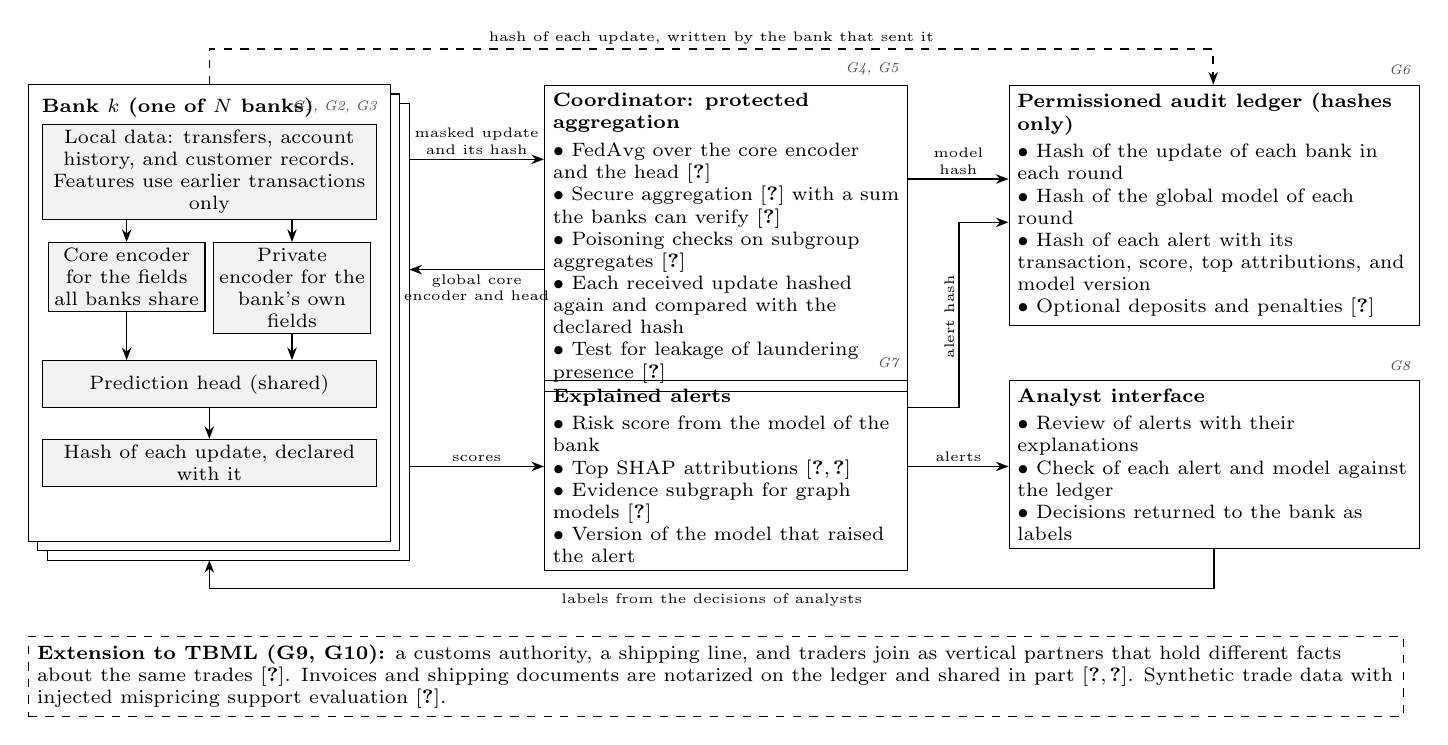
\begin{tikzpicture}[font=\scriptsize,
  blk/.style={draw, rectangle, align=flush left, inner sep=3pt, anchor=north west},
  sub/.style={draw, rectangle, fill=gray!10, align=flush center, inner sep=2pt, minimum height=6mm, anchor=north},
  arr/.style={-{Stealth[length=1.6mm]}, semithick},
  lab/.style={font=\tiny, align=flush center, inner sep=1.5pt},
  gap/.style={font=\tiny\itshape, text=black!70, anchor=north east}]
% stack of banks: two shadow copies behind the front box
\draw[fill=white] (0.24,-0.24) rectangle (4.84,-6.04);
\draw[fill=white] (0.12,-0.12) rectangle (4.72,-5.92);
\draw[fill=white] (0,0) rectangle (4.6,-5.8);
\coordinate (bank) at (2.3,-2.9);
\node[anchor=north west, font=\scriptsize\bfseries] at (0.05,-0.05) {Bank $k$ (one of $N$ banks)};
\node[gap] at (4.55,-0.09) {G1, G2, G3};
\node[sub, text width=4.1cm] (data) at (2.3,-0.5) {Local data: transfers, account history, and customer records. Features use earlier transactions only};
\node[sub, text width=1.85cm] (core) at (1.25,-2.0) {Core encoder for the fields all banks share};
\node[sub, text width=1.85cm] (priv) at (3.35,-2.0) {Private encoder for the bank's own fields};
\node[sub, text width=4.1cm] (headn) at (2.3,-3.5) {Prediction head (shared)};
\node[sub, text width=4.1cm] (hashn) at (2.3,-4.5) {Hash of each update, declared with it};
\draw[arr] (data.south -| core.north) -- (core.north);
\draw[arr] (data.south -| priv.north) -- (priv.north);
\draw[arr] (core.south) -- (core.south |- headn.north);
\draw[arr] (priv.south) -- (priv.south |- headn.north);
\draw[arr] (headn) -- (hashn);
% coordinator
\node[blk, text width=4.4cm] (coord) at (6.55,0) {\textbf{Coordinator: protected aggregation}\\[2pt]
$\bullet$ FedAvg over the core encoder and the head \cite{mcmahan2017fedavg}\\
$\bullet$ Secure aggregation \cite{bonawitz2017secagg} with a sum the banks can verify \cite{wang2023vosa}\\
$\bullet$ Poisoning checks on subgroup aggregates \cite{zhang2023safelearning}\\
$\bullet$ Each received update hashed again and compared with the declared hash\\
$\bullet$ Test for leakage of laundering presence \cite{gao2023category}};
\node[gap, anchor=south east] at (coord.north east) {G4, G5};
% ledger
\node[blk, text width=5.0cm] (ledger) at (12.45,0) {\textbf{Permissioned audit ledger (hashes only)}\\[2pt]
$\bullet$ Hash of the update of each bank in each round\\
$\bullet$ Hash of the global model of each round\\
$\bullet$ Hash of each alert with its transaction, score, top attributions, and model version\\
$\bullet$ Optional deposits and penalties \cite{yang2022accountable}};
\node[gap, anchor=south east] at (ledger.north east) {G6};
% explained alerts
\node[blk, text width=4.4cm] (alerts) at (6.55,-3.75) {\textbf{Explained alerts}\\[2pt]
$\bullet$ Risk score from the model of the bank\\
$\bullet$ Top SHAP attributions \cite{lundberg2017shap,awosika2024xai}\\
$\bullet$ Evidence subgraph for graph models \cite{nayak2026quantum}\\
$\bullet$ Version of the model that raised the alert};
\node[gap, anchor=south east] at (alerts.north east) {G7};
% analyst interface
\node[blk, text width=5.0cm] (analyst) at (12.45,-3.75) {\textbf{Analyst interface}\\[2pt]
$\bullet$ Review of alerts with their explanations\\
$\bullet$ Check of each alert and model against the ledger\\
$\bullet$ Decisions returned to the bank as labels};
\node[gap, anchor=south east] at (analyst.north east) {G8};
% arrows between components
\coordinate (ymh) at (0,-1.2);
\coordinate (yal) at (0,-4.85);
\coordinate (yah) at (0,-4.1);
\coordinate (ylb) at (0,-6.4);
\draw[arr] (4.84,-0.95) -- node[lab, above] {masked update\\and its hash} (6.55,-0.95);
\draw[arr] (6.55,-2.35) -- node[lab, below] {global core\\encoder and head} (4.84,-2.35);
\draw[arr] (coord.east |- ymh) -- node[lab, above] {model\\hash} (12.45,-1.2);
\draw[arr] (4.84,-4.85) -- node[lab, above] {scores} (6.55,-4.85);
\draw[arr] (alerts.east |- yal) -- node[lab, above] {alerts} (12.45,-4.85);
\draw[arr] (alerts.east |- yah) -- (11.82,-4.1) -- (11.82,-1.75) -- (12.45,-1.75);
\node[lab, rotate=90, anchor=south] at (11.82,-2.95) {alert hash};
\draw[arr, dashed] (2.3,0) -- (2.3,0.45) -- node[lab, above] {hash of each update, written by the bank that sent it} (15.05,0.45) -- (15.05,0);
\draw[arr] (analyst.south) -- (analyst.south |- ylb) -- node[lab, below] {labels from the decisions of analysts} (2.3,-6.4) -- (2.3,-6.04);
% extension to trade
\node[draw, dashed, anchor=north west, text width=17.25cm, align=flush left, inner sep=3pt] (tbml) at (0,-7.0) {\textbf{Extension to TBML (G9, G10):} a customs authority, a shipping line, and traders join as vertical partners that hold different facts about the same trades \cite{li2026plc}. Invoices and shipping documents are notarized on the ledger and shared in part \cite{dudczyk2024supply,cosmin2024notary}. Synthetic trade data with injected mispricing support evaluation \cite{altman2023ibmaml}.};
\end{tikzpicture}
\caption{Reference architecture for detecting laundering across banks with private data, protected aggregation, a ledger of hashes, and explained alerts. Labels G1 to G10 mark the research gaps that each component addresses.}
\label{fig:arch}
\end{figure*}

The findings suggest the architecture shown in Fig.~\ref{fig:arch}. Each component is grounded in a technique from the corpus, while the whole addresses gaps G1 to G8, and its extension to trade addresses G9 and G10.

\begin{itemize}
\item \textbf{Bank nodes.} Each bank keeps its transfers and customer records. It computes the core fields that every bank sees for its own payments, such as the amount, the currencies, the payment format, and the time. It adds its own features from account history and its own customer attributes. Features use only earlier transactions, and evaluation splits the data by time as in \cite{mao2026pmegnn,nayak2026quantum} (G3).
\item \textbf{Hybrid federated model.} The model has three parts. A core encoder reads the fields that all banks share, a private encoder reads the fields of one bank, and a prediction head combines both. The core encoder and the head are averaged with FedAvg \cite{mcmahan2017fedavg}, while each private encoder stays at its bank. This extends the input layers per bank of \cite{tang2024sdt} and avoids the matching of customers that vertical FL requires \cite{li2026plc} (G1, G2).
\item \textbf{Protected aggregation.} Updates are combined with secure aggregation \cite{bonawitz2017secagg} that lets the banks verify the aggregate \cite{wang2023vosa} and checks subgroup aggregates for poisoning \cite{zhang2023safelearning}. The category inference attack of \cite{gao2023category} serves as a test of whether the presence of laundering cases at a bank leaks (G4, G5).
\item \textbf{Audit ledger.} A permissioned chain run by the participating banks and the supervisor records hashes only. Each bank writes the hash of the update it sends, and the coordinator writes the hash of every aggregated model. Before aggregating, the coordinator hashes each update it received again and stops if the result differs from the declared hash. Deposits and penalties as in \cite{yang2022accountable} can be added (G6).
\item \textbf{Explained alerts.} Every alert carries a score and its top SHAP attributions \cite{lundberg2017shap,awosika2024xai}, and for graph models an evidence subgraph \cite{nayak2026quantum}. The transaction identifier, the score, the attributions, and the model version are hashed together and written to the ledger, so that an auditor can later verify that an alert came from a recorded model and has not been altered (G7).
\item \textbf{Analyst interface.} Analysts review alerts with their explanations, check the ledger record of each alert and model, and return their decisions to the bank as new labels (G8).
\end{itemize}

The authors have implemented a prototype of the bank nodes, the hybrid federated model, the audit ledger, and the explained alerts, together with a dashboard for analysts, on the IBM HI-Small data \cite{altman2023ibmaml}. Transfers are assigned to five simulated banks by sending bank, and each bank holds a different set of features from account history and of synthetic customer attributes. Protected aggregation and the extension to trade are not yet part of the prototype, and its evaluation is outside the scope of this review.

A research agenda follows from the architecture. In the near term, FL on laundering data should be evaluated under a common protocol against models trained by each bank alone and a model trained on pooled data. The protocol would use splits by time, the area under the precision recall curve, recall for each laundering typology, and several seeds (G1, G3). Next, the leakage of laundering presence through aggregation should be measured and bounded, and defenses for verification and poisoning should be tested with financial models (G4, G5). In parallel, explanations should be assessed with analysts and stored with the version of the model that produced them (G7). Finally, the architecture extends to TBML when customs authorities and shipping lines join as vertical partners that hold different facts about the same trades \cite{li2026plc}, with trade documents verified on the ledger \cite{dudczyk2024supply,cosmin2024notary} (G9, G10). A simulator of trade with injected mispricing, built in the way the IBM transactions were generated \cite{altman2023ibmaml}, would make this extension measurable.

\section{Threats to Validity}
\label{sec:validity}

\emph{Selection bias.} The corpus comes from a targeted search organized into four clusters, mainly in IEEE Xplore, rather than an exhaustive search of several databases. Relevant work in ACM, Elsevier, Springer, and preprint venues may be missing, including FL studies on laundering data that would change the answer to RQ2. The number of records screened before full-text retrieval was not logged, so Fig.~\ref{fig:prisma} starts from the collected files. One study could not be retrieved because its file contained another paper.

\emph{Size and recency.} With 27 studies the review is small, and categories of two to six studies support only tentative conclusions. Two thirds of the corpus was published in 2024 or later, and several articles were published online before their final issue, so their final versions may differ.

\emph{Extraction and classification.} Bibliographic data were taken from each PDF, and numbers were copied as printed and checked against the source. Where tables were available only as images, the relative improvements stated in the text were used instead \cite{luo2024mlad}. Each study was assigned one primary category, although several span two or more, and the grading of relevance involves judgment.

\emph{Synthesis.} Differences in datasets, splits, metrics, and baselines ruled out a meta-analysis, and Section~\ref{sec:comparability} shows that the reported numbers cannot be ranked across studies. Several results rest on synthetic data \cite{amber2026cbdc,mao2026pmegnn} or on a single dataset \cite{luo2024mlad}.

\section{Conclusion}
\label{sec:conclusion}

This review examined 27 studies on detecting laundering and fraud, training models across institutions, protecting that training, and auditing it with blockchain. Graph models are the most active line of work. They show that the structure of payment networks, the direction of payments, and the features of neighbors all improve detection, and they report strong numbers on Elliptic and on the IBM data. Those numbers cannot be compared across studies because data, splits, and metrics differ, and accuracy is still reported despite the extreme imbalance of laundering.

Collaboration is the weak point. Only three studies train fraud detectors across institutions, none on laundering data, and only one lets institutions keep different columns without matching customers. The secure aggregation schemes in the corpus can verify aggregates, tolerate dropouts, detect backdoors, and penalize cheating. No scheme does all of these, and none has been tested on a financial model. Secure aggregation also still reveals which classes a participant holds. Blockchain is used for incentives, accountability, policies, and documents, but not yet to record the life cycle of a detection model and its alerts. Explanations are produced but neither assessed nor tied to the model that made them. TBML detection is still limited to price statistics, mirror analysis, and a single classifier.

The reference architecture proposed here pairs a hybrid federated model for banks with different schemas with protected aggregation. A ledger keeps the hashes of updates, models, and alerts, and every explanation is bound to the version of the model that produced it. Extending it to customs and shipping data is the path from monitoring transactions to detecting trade-based laundering.

\section*{Author Contributions}

A.N., A.S., and L.S. contributed equally to the literature search and screening, data extraction and classification, synthesis of findings, preparation of figures and tables, and writing of the manuscript. S.R.K. supervised the work and reviewed the manuscript.

\section*{Acknowledgment}

The authors thank the Department of Computer Engineering, Modern Education Society's Wadia College of Engineering, Pune, for access to the digital library resources used in this review.

\appendices

\section{Classification of the Reviewed Corpus}

Table~\ref{tab:corpus} lists all 27 reviewed studies with their year, venue type, search cluster, primary category, relevance grade, and principal contribution. The studies are grouped by category.

\begin{table*}[!t]
\centering
\caption{Classification of the 27 Reviewed Studies by Primary Category (Type C: Conference, J: Journal. Cluster A: Anti-Money Laundering, G: Graph and Machine Learning, F: Federated Learning, B: Blockchain. Relevance H, M, or L)}
\label{tab:corpus}
\footnotesize
\begin{tabularx}{\textwidth}{@{}L{0.7cm}L{2.45cm}cccL{3.0cm}cY@{}}
\toprule
\textbf{Ref.} & \textbf{Study} & \textbf{Year} & \textbf{Type} & \textbf{Cluster} & \textbf{Category} & \textbf{Rel.} & \textbf{Principal contribution}\\
\midrule
\cite{jensen2023fighting} & Fighting money laundering & 2023 & J & G & AML and TBML reviews & H & Terminology of client risk profiling and suspicious behavior flagging, call for public data and PR curves\\
\cite{tiwari2025tbml} & TBML review & 2025 & J & A & AML and TBML reviews & H & First systematic review of TBML, four themes, detection limited to price and mirror statistics\\
\cite{raj2024ai} & AI in AML & 2024 & C & A & AML and TBML reviews & L & Narrative account of AI in KYC, due diligence, and monitoring\\
\midrule
\cite{ferretti2025gnn} & GNNs on Elliptic & 2025 & J & G & Graph and machine learning detection & H & Chebyshev and attention networks with a final linear layer and skip connections\\
\cite{irshad2024gcfmld} & GCF-MLD & 2024 & J & G & Graph and machine learning detection & H & Graph features with K-means and hierarchical clustering on alerts of a real bank\\
\cite{luo2024mlad} & MLaD$^2$ & 2024 & J & G & Graph and machine learning detection & H & Similarity graph of accounts with contrastive pretraining and supervised tuning\\
\cite{mao2026pmegnn} & PME-GNN & 2026 & C & G & Graph and machine learning detection & H & Neighbourhood aggregation with random walk encoding, messages in both directions, and sparse experts on IBM data\\
\cite{nayak2026quantum} & Quantum-Enhanced AML & 2026 & J & G & Graph and machine learning detection & H & Entity resolution, temporal contrastive learning, a quantum layer, and evidence subgraphs\\
\cite{yu2023aetransgat} & AEtransGAT & 2023 & C & G & Graph and machine learning detection & H & Graph attention weighted by amount with an autoencoder trained through mutual learning\\
\midrule
\cite{wu2024heists} & XBlockFlow & 2024 & J & A & Cryptocurrency and CBDC laundering & H & Tracing from 73 Ethereum incidents and the EthereumHeist dataset\\
\cite{amber2026cbdc} & CBDC integrity & 2026 & J & A, B, G & Cryptocurrency and CBDC laundering & H & Smart contracts, taint analysis, and classifiers for a CBDC on synthetic data\\
\midrule
\cite{tang2024sdt} & SDT with FL & 2024 & J & A, F & FL for financial fraud & H & Structured data transformer federated across two banks with different features\\
\cite{awosika2024xai} & FL and XAI & 2024 & J & B, F & FL for financial fraud & H & Federated dense network with SHAP on bank account fraud\\
\cite{li2026plc} & PLC & 2026 & J & F & FL for financial fraud & H & Joint horizontal and vertical FL with sparse secure aggregation\\
\midrule
\cite{yang2022accountable} & Accountable aggregation & 2022 & J & F & Secure aggregation and attacks & M & Homomorphic proxy aggregation with deposits and penalties on a blockchain\\
\cite{zhang2023safelearning} & SAFELearning & 2023 & J & F & Secure aggregation and attacks & M & Secure aggregation with oblivious grouping that still detects backdoors\\
\cite{gao2023category} & Category inference & 2023 & J & F & Secure aggregation and attacks & M & Attack that reveals the classes each client holds despite secure aggregation\\
\cite{sami2024tinysecagg} & TinySecAgg & 2024 & J & F & Secure aggregation and attacks & M & Sparsified secure aggregation that also hides coordinates\\
\cite{wang2023vosa} & VOSA & 2023 & J & F & Secure aggregation and attacks & M & Verifiable aggregation that tolerates dropouts\\
\midrule
\cite{ahmed2024bcfl} & BCFL for crypto fraud & 2024 & J & B, F & Blockchain for FL and machine learning & H & Review of blockchain FL architectures, consensus, and scalability for cryptocurrency fraud\\
\cite{xiong2025hppbefl} & HPP-BEFL & 2025 & J & B & Blockchain for FL and machine learning & M & Group key agreement across heterogeneous public key systems for blockchain FL\\
\cite{ural2023bcml} & Blockchain for ML survey & 2023 & J & B, G & Blockchain for FL and machine learning & M & Survey of blockchain for securing, validating, and sharing machine learning\\
\cite{li2021befl} & Blockchain FL survey & 2021 & C & B & Blockchain for FL and machine learning & L & Framework of six layers for FL on a blockchain\\
\midrule
\cite{chen2024finance} & Blockchain in finance & 2024 & J & B & Blockchain for financial records, trade, and documents & M & Trust, data management, and automation in finance, including AML audit trails\\
\cite{dudczyk2024supply} & Supply chain survey & 2024 & J & B & Blockchain for financial records, trade, and documents & L & Blockchain in global supply chains, including customs and trade data\\
\cite{cosmin2024notary} & Digital notarization & 2024 & J & B & Blockchain for financial records, trade, and documents & L & Microservices for notarizing and partially sharing documents with IPFS and a blockchain\\
\cite{kapadiya2022health} & Health insurance fraud & 2022 & J & B & Blockchain for financial records, trade, and documents & L & Blockchain and AI architecture for health insurance fraud\\
\bottomrule
\end{tabularx}
\end{table*}

\begin{thebibliography}{99}

\bibitem{raj2024ai}
M. Raj, Y. Chanti, H. Khan, M. Sahu, and S. Kathuria, ``The Use of Artificial Intelligence in Anti-Money Laundering (AML),'' in \emph{Proc. 3rd Int. Conf. Sentiment Analysis and Deep Learning (ICSADL)}, 2024, pp. 272--277, doi: 10.1109/ICSADL61749.2024.00050.

\bibitem{jensen2023fighting}
R. I. T. Jensen and A. Iosifidis, ``Fighting Money Laundering With Statistics and Machine Learning,'' \emph{IEEE Access}, vol. 11, 2023, pp. 8889--8903, doi: 10.1109/ACCESS.2023.3239549.

\bibitem{fatf2006tbml}
Financial Action Task Force, ``Trade-based money laundering,'' FATF/OECD, Paris, France, 2006.

\bibitem{tiwari2025tbml}
M. Tiwari, J. Ferrill, and D. M. C. Allan, ``Trade-based money laundering: a systematic literature review,'' \emph{J. Accounting Literature}, vol. 47, no. 5, 2025, pp. 1--26, doi: 10.1108/JAL-11-2022-0111.

\bibitem{awosika2024xai}
T. Awosika, R. M. Shukla, and B. Pranggono, ``Transparency and Privacy: The Role of Explainable AI and Federated Learning in Financial Fraud Detection,'' \emph{IEEE Access}, vol. 12, 2024, pp. 64551--64560, doi: 10.1109/ACCESS.2024.3394528.

\bibitem{irshad2024gcfmld}
F. Irshad, T. Alkhalifah, F. Alturise, and Y. D. Khan, ``GCF-MLD: Integrated Approach for Money Laundering Detection Using Machine Learning and Graph Network Analysis,'' \emph{IEEE Access}, vol. 12, 2024, pp. 183961--183972, doi: 10.1109/ACCESS.2024.3510115.

\bibitem{luo2024mlad}
X. Luo, X. Han, W. Zuo, X. Wu, and W. Liu, ``MLaD$^2$: A Semi-Supervised Money Laundering Detection Framework Based on Decoupling Training,'' \emph{IEEE Trans. Inf. Forensics Security}, vol. 19, 2024, pp. 4518--4533, doi: 10.1109/TIFS.2024.3380262.

\bibitem{ferretti2025gnn}
S. Ferretti, G. D'Angelo, and V. Ghini, ``Enhancing Anti-Money Laundering Frameworks: An Application of Graph Neural Networks in Cryptocurrency Transaction Classification,'' \emph{IEEE Access}, vol. 13, 2025, pp. 50201--50215, doi: 10.1109/ACCESS.2025.3552240.

\bibitem{mao2026pmegnn}
M. Mao, Q. Zhou, and X. Yu, ``PME-GNN: Graph Neural Networks for Anti-Money Laundering Detection,'' in \emph{Proc. IEEE 5th Int. Conf. Information Technology, Big Data and Artificial Intelligence (ICIBA)}, 2026, pp. 1041--1044, doi: 10.1109/ICIBA68339.2026.11651713.

\bibitem{amber2026cbdc}
S. T. Amber, H. Ghafoor, P. D. Thanh, and C.-H. Hsia, ``Reinforcing CBDC Integrity: A Novel Anti Money Laundering Solution by Integrating Blockchain, Machine Learning, and Taint Analysis,'' \emph{IEEE Open J. Comput. Soc.}, vol. 7, 2026, pp. 514--527, doi: 10.1109/OJCS.2026.3666199.

\bibitem{yu2023aetransgat}
L. Yu, F. Zhang, J. Ma, L. Yang, Y. Yang, and W. Jia, ``Who Are the Money Launderers? Money Laundering Detection on Blockchain via Mutual Learning-Based Graph Neural Network,'' in \emph{Proc. Int. Joint Conf. Neural Networks (IJCNN)}, 2023, doi: 10.1109/IJCNN54540.2023.10191217.

\bibitem{mcmahan2017fedavg}
B. McMahan, E. Moore, D. Ramage, S. Hampson, and B. A. y Arcas, ``Communication-efficient learning of deep networks from decentralized data,'' in \emph{Proc. 20th Int. Conf. Artificial Intelligence and Statistics (AISTATS)}, 2017, pp. 1273--1282.

\bibitem{bonawitz2017secagg}
K. Bonawitz \emph{et al.}, ``Practical secure aggregation for privacy-preserving machine learning,'' in \emph{Proc. ACM SIGSAC Conf. Computer and Communications Security (CCS)}, 2017, pp. 1175--1191.

\bibitem{chen2024finance}
H. Chen, N. Wei, L. Wang, W. F. M. Mobarak, M. A. Albahar, and Z. A. Shaikh, ``The Role of Blockchain in Finance Beyond Cryptocurrency: Trust, Data Management, and Automation,'' \emph{IEEE Access}, vol. 12, 2024, pp. 64861--64885, doi: 10.1109/ACCESS.2024.3395918.

\bibitem{yang2022accountable}
X. Yang, Y. Zhao, Q. Chen, Y. Yu, X. Du, and M. Guizani, ``Accountable and Verifiable Secure Aggregation for Federated Learning in IoT Networks,'' \emph{IEEE Netw.}, vol. 36, no. 5, 2022, pp. 173--179, doi: 10.1109/MNET.001.2200214.

\bibitem{ahmed2024bcfl}
A. A. Ahmed and O. O. Alabi, ``Secure and Scalable Blockchain-Based Federated Learning for Cryptocurrency Fraud Detection: A Systematic Review,'' \emph{IEEE Access}, vol. 12, 2024, pp. 102219--102241, doi: 10.1109/ACCESS.2024.3429205.

\bibitem{li2021befl}
C. Li, Y. Yuan, and F.-Y. Wang, ``Blockchain-enabled Federated Learning: A Survey,'' in \emph{Proc. IEEE 1st Int. Conf. Digital Twins and Parallel Intelligence (DTPI)}, 2021, pp. 286--289, doi: 10.1109/DTPI52967.2021.9540163.

\bibitem{ural2023bcml}
O. Ural and K. Yoshigoe, ``Survey on Blockchain-Enhanced Machine Learning,'' \emph{IEEE Access}, vol. 11, 2023, pp. 145331--145362, doi: 10.1109/ACCESS.2023.3344669.

\bibitem{page2021prisma}
M. J. Page \emph{et al.}, ``The PRISMA 2020 statement: An updated guideline for reporting systematic reviews,'' \emph{BMJ}, vol. 372, Art. no. n71, 2021, doi: 10.1136/bmj.n71.

\bibitem{weber2019elliptic}
M. Weber \emph{et al.}, ``Anti-money laundering in Bitcoin: Experimenting with graph convolutional networks for financial forensics,'' in \emph{Proc. KDD Workshop on Anomaly Detection in Finance}, 2019, arXiv:1908.02591.

\bibitem{altman2023ibmaml}
E. Altman, J. Blanu\v{s}a, L. von Nieder\"ausern, B. Egressy, A. Anghel, and K. Atasu, ``Realistic synthetic financial transactions for anti-money laundering models,'' in \emph{Proc. Advances in Neural Information Processing Systems (NeurIPS)}, vol. 36, 2023, pp. 29851--29874.

\bibitem{wu2024heists}
J. Wu \emph{et al.}, ``Toward Understanding Asset Flows in Crypto Money Laundering Through the Lenses of Ethereum Heists,'' \emph{IEEE Trans. Inf. Forensics Security}, vol. 19, 2024, pp. 1994--2009, doi: 10.1109/TIFS.2023.3346276.

\bibitem{zdanowicz2009}
J. S. Zdanowicz, ``Trade-based money laundering and terrorist financing,'' \emph{Rev. Law Econ.}, vol. 5, no. 2, 2009, pp. 855--878, doi: 10.2202/1555-5879.1419.

\bibitem{dudczyk2024supply}
P. Dudczyk, J. K. Dunston, and G. V. Crosby, ``Blockchain Technology for Global Supply Chain Management: A Survey of Applications, Challenges, Opportunities and Implications,'' \emph{IEEE Access}, vol. 12, 2024, pp. 70065--70088, doi: 10.1109/ACCESS.2024.3399759.

\bibitem{li2026plc}
Z. Li, Y. Kong, and C. Jiang, ``Privacy-Aware Transaction Fraud Detection With Low Communication Costs Under Joint Federated Learning,'' \emph{IEEE Trans. Dependable Secure Comput.}, vol. 23, no. 3, 2026, pp. 4511--4525, doi: 10.1109/TDSC.2025.3647476.

\bibitem{sami2024tinysecagg}
H. U. Sami and B. G\"uler, ``Secure Gradient Aggregation With Sparsification for Resource-Limited Federated Learning,'' \emph{IEEE Trans. Commun.}, vol. 72, no. 11, 2024, pp. 6883--6899, doi: 10.1109/TCOMM.2024.3403475.

\bibitem{xiong2025hppbefl}
H. Xiong, Y. Xia, Y. Zhao, A. Wahaballa, and K.-H. Yeh, ``Heterogeneous Privacy-Preserving Blockchain-Enabled Federated Learning for Social Fintech,'' \emph{IEEE Trans. Comput. Social Syst.}, vol. 12, no. 6, 2025, pp. 5229--5244, doi: 10.1109/TCSS.2025.3533634.

\bibitem{kapadiya2022health}
K. Kapadiya \emph{et al.}, ``Blockchain and AI-Empowered Healthcare Insurance Fraud Detection: An Analysis, Architecture, and Future Prospects,'' \emph{IEEE Access}, vol. 10, 2022, pp. 79606--79627, doi: 10.1109/ACCESS.2022.3194569.

\bibitem{kitchenham2007}
B. Kitchenham and S. Charters, ``Guidelines for performing systematic literature reviews in software engineering,'' Keele Univ. and Durham Univ., Tech. Rep. EBSE-2007-01, 2007.

\bibitem{tang2024sdt}
Y. Tang and Z. Liu, ``A Credit Card Fraud Detection Algorithm Based on SDT and Federated Learning,'' \emph{IEEE Access}, vol. 12, 2024, pp. 182547--182560, doi: 10.1109/ACCESS.2024.3491175.

\bibitem{nayak2026quantum}
S. Nayak and R. Kumar, ``Quantum-Enhanced AML: Hybrid Quantum--Classical Graph Learning With Entity Resolution and Evidence Subgraph Discovery for Transaction Screening,'' \emph{IEEE Access}, vol. 14, 2026, pp. 74837--74850, doi: 10.1109/ACCESS.2026.3692342.

\bibitem{cosmin2024notary}
I. Cosmin-Iulian and I. Adrian, ``Decentralized Infrastructure for Digital Notarizing, Signing, and Sharing Documents Securely Using Microservices and Blockchain,'' \emph{IEEE Access}, vol. 12, 2024, pp. 195816--195829, doi: 10.1109/ACCESS.2024.3518977.

\bibitem{wang2023vosa}
Y. Wang, A. Zhang, S. Wu, and S. Yu, ``VOSA: Verifiable and Oblivious Secure Aggregation for Privacy-Preserving Federated Learning,'' \emph{IEEE Trans. Dependable Secure Comput.}, vol. 20, no. 5, 2023, pp. 3601--3616, doi: 10.1109/TDSC.2022.3226508.

\bibitem{zhang2023safelearning}
Z. Zhang, J. Li, S. Yu, and C. Makaya, ``SAFELearning: Secure Aggregation in Federated Learning With Backdoor Detectability,'' \emph{IEEE Trans. Inf. Forensics Security}, vol. 18, 2023, pp. 3289--3304, doi: 10.1109/TIFS.2023.3280032.

\bibitem{gao2023category}
J. Gao \emph{et al.}, ``Secure Aggregation is Insecure: Category Inference Attack on Federated Learning,'' \emph{IEEE Trans. Dependable Secure Comput.}, vol. 20, no. 1, 2023, pp. 147--160, doi: 10.1109/TDSC.2021.3128679.

\bibitem{egressy2024multignn}
B. Egressy, L. von Nieder\"ausern, J. Blanu\v{s}a, E. Altman, R. Wattenhofer, and K. Atasu, ``Provably powerful graph neural networks for directed multigraphs,'' in \emph{Proc. AAAI Conf. Artificial Intelligence}, vol. 38, no. 10, 2024, pp. 11838--11846.

\bibitem{jesus2022baf}
S. Jesus \emph{et al.}, ``Turning the tables: Biased, imbalanced, dynamic tabular datasets for ML evaluation,'' in \emph{Proc. Advances in Neural Information Processing Systems (NeurIPS)}, vol. 35, 2022.

\bibitem{lundberg2017shap}
S. M. Lundberg and S.-I. Lee, ``A unified approach to interpreting model predictions,'' in \emph{Proc. Advances in Neural Information Processing Systems (NIPS)}, vol. 30, 2017, pp. 4765--4774.

\end{thebibliography}

\end{document}
